

\documentclass[10pt,xcolor=dvipsnames]{beamer}\usepackage[]{graphicx}\usepackage[]{color}
%% maxwidth is the original width if it is less than linewidth
%% otherwise use linewidth (to make sure the graphics do not exceed the margin)
\makeatletter
\def\maxwidth{ %
  \ifdim\Gin@nat@width>\linewidth
    \linewidth
  \else
    \Gin@nat@width
  \fi
}
\makeatother

\definecolor{fgcolor}{rgb}{0.345, 0.345, 0.345}
\newcommand{\hlnum}[1]{\textcolor[rgb]{0.686,0.059,0.569}{#1}}%
\newcommand{\hlstr}[1]{\textcolor[rgb]{0.192,0.494,0.8}{#1}}%
\newcommand{\hlcom}[1]{\textcolor[rgb]{0.678,0.584,0.686}{\textit{#1}}}%
\newcommand{\hlopt}[1]{\textcolor[rgb]{0,0,0}{#1}}%
\newcommand{\hlstd}[1]{\textcolor[rgb]{0.345,0.345,0.345}{#1}}%
\newcommand{\hlkwa}[1]{\textcolor[rgb]{0.161,0.373,0.58}{\textbf{#1}}}%
\newcommand{\hlkwb}[1]{\textcolor[rgb]{0.69,0.353,0.396}{#1}}%
\newcommand{\hlkwc}[1]{\textcolor[rgb]{0.333,0.667,0.333}{#1}}%
\newcommand{\hlkwd}[1]{\textcolor[rgb]{0.737,0.353,0.396}{\textbf{#1}}}%
\let\hlipl\hlkwb

\usepackage{framed}
\makeatletter
\newenvironment{kframe}{%
 \def\at@end@of@kframe{}%
 \ifinner\ifhmode%
  \def\at@end@of@kframe{\end{minipage}}%
  \begin{minipage}{\columnwidth}%
 \fi\fi%
 \def\FrameCommand##1{\hskip\@totalleftmargin \hskip-\fboxsep
 \colorbox{shadecolor}{##1}\hskip-\fboxsep
     % There is no \\@totalrightmargin, so:
     \hskip-\linewidth \hskip-\@totalleftmargin \hskip\columnwidth}%
 \MakeFramed {\advance\hsize-\width
   \@totalleftmargin\z@ \linewidth\hsize
   \@setminipage}}%
 {\par\unskip\endMakeFramed%
 \at@end@of@kframe}
\makeatother

\definecolor{shadecolor}{rgb}{.97, .97, .97}
\definecolor{messagecolor}{rgb}{0, 0, 0}
\definecolor{warningcolor}{rgb}{1, 0, 1}
\definecolor{errorcolor}{rgb}{1, 0, 0}
\newenvironment{knitrout}{}{} % an empty environment to be redefined in TeX

\usepackage{alltt}
\setbeamertemplate{navigation symbols}{}



\usepackage{color}
\usepackage{CREAL_slides}
\usepackage[latin1]{inputenc}
\usepackage{calc}
\usepackage[loadonly]{enumitem}
\usepackage{float}
\usepackage[position=top,singlelinecheck=off]{subfig}
\usepackage{amsfonts}
\usepackage{amssymb}
\usepackage{amsmath}
\usepackage{tikz}
\usetikzlibrary{arrows}

\DeclareMathOperator{\argmax}{arg\,max}

\newcommand{\X}{\mathbf{X}}



\title[Multivariate methods in health studies]{Unsupervised Methods}
\author[Juan R Gonzalez]{Juan R Gonzalez}
\institute[ISGlobal]{BRGE - Bioinformatics Research Group in Epidemiology \\
		  Barcelona Institute for Global Health (ISGlobal) \\
		           {\tt e-mail:juanr.gonzalez@isglobal.org} \\
                  \url{http://brge.isglobal.org} \\
                  and Departament of Mathematics, UAB
                  }

\date{}
\IfFileExists{upquote.sty}{\usepackage{upquote}}{}
\begin{document}






\frame{\titlepage}




\begin{frame}{Outline}
\tableofcontents
\end{frame}


%%%%%%%%%%%%%%%%%%%%%%%%%%%%%%%%%%%%
\section{Multidimensional reduction}
%%%%%%%%%%%%%%%%%%%%%%%%%%%%%%%%%%%%

%%%%%%%%%%%%%%%%%%%%%%%%%%%%%%%%%%%%%%%%%
\subsection{Principal component analysis}
%%%%%%%%%%%%%%%%%%%%%%%%%%%%%%%%%%%%%%%%%

\begin{frame}[plain]{Principal component analysis}

\begin{itemize}
 \item The goal is to find a small number of independent linear combinations (principal components) of a set 
of measured variables that capture as much 
of the variability in the original variables as 
possible. 
 \item  Supplementary variables can also be considered. They are not included in the calculation of principal components and including them does not affect the results. The supplementary variables are projected on to the loading plot and used to enhance interpretation.
 \item It is a useful exploratory technique 
and can help you to create predictive models. For instance, in disease association studies, principal components are regressed against health outcomes.
\end{itemize}

\end{frame}

\begin{frame}[plain]\frametitle{Principal component analysis}

\begin{figure}
\begin{center}
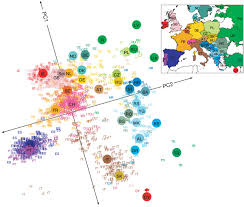
\includegraphics[height=5cm, width=5cm]{figures/pca_example.jpg}
\end{center}
\end{figure}

\end{frame}



\begin{frame}[plain]\frametitle{Principal component analysis}

\begin{itemize}
\item It is used in genomic, transcriptomic or epidemiological studies to find patterns (signatures) with regard to variantes, abundance of mRNAs or exposure/diet, respectively.
\item Given a data set $X$, which is a $n \times p$ matrix, of $n$ individuals and $p$ features
$$ X=(x_1, x_2, \ldots, x_p)$$ 
  \item we look for new variables that are linear combinations of the original variables
$f=q_1X_1 + q_2X_2 + \ldots + q_pX_p$  or $f=Xq$ where $q$ are know as loadings.
\item We introduce the restriction that for $i$th component, $q$'s should maximize the variance components of $f$'s
$$ \argmax_{q^i} \text{var}(Xq^i)$$ and $q$'s has to be orthogonal to each other.
\end{itemize}

\end{frame}

\begin{frame}[fragile, plain]\frametitle{Principal component analysis}

\begin{knitrout}\footnotesize
\definecolor{shadecolor}{rgb}{0.969, 0.969, 0.969}\color{fgcolor}

{\centering 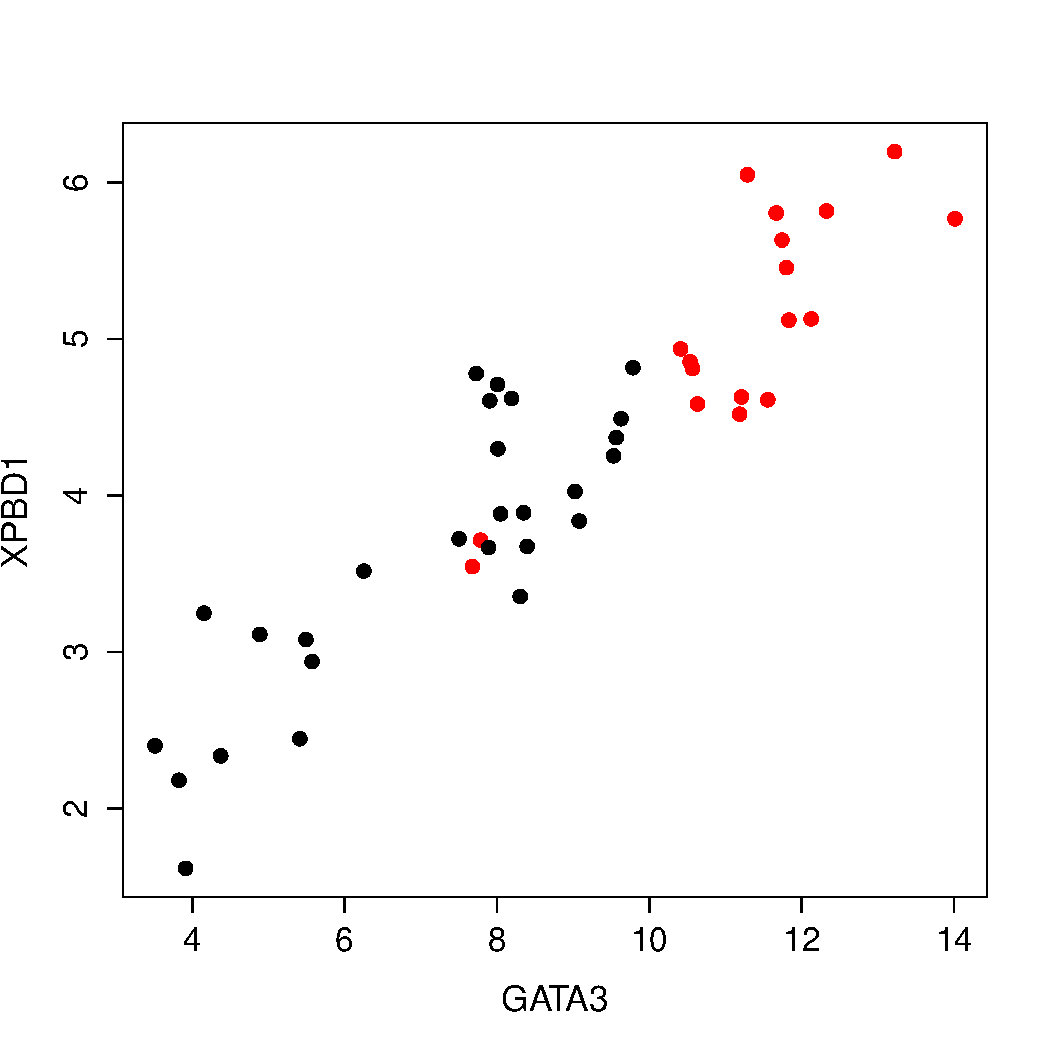
\includegraphics[width=2in]{figure/plot_pca_1-1} 

}



\end{knitrout}

\end{frame}

\begin{frame}[fragile, plain]\frametitle{Principal component analysis}

\begin{knitrout}\footnotesize
\definecolor{shadecolor}{rgb}{0.969, 0.969, 0.969}\color{fgcolor}

{\centering 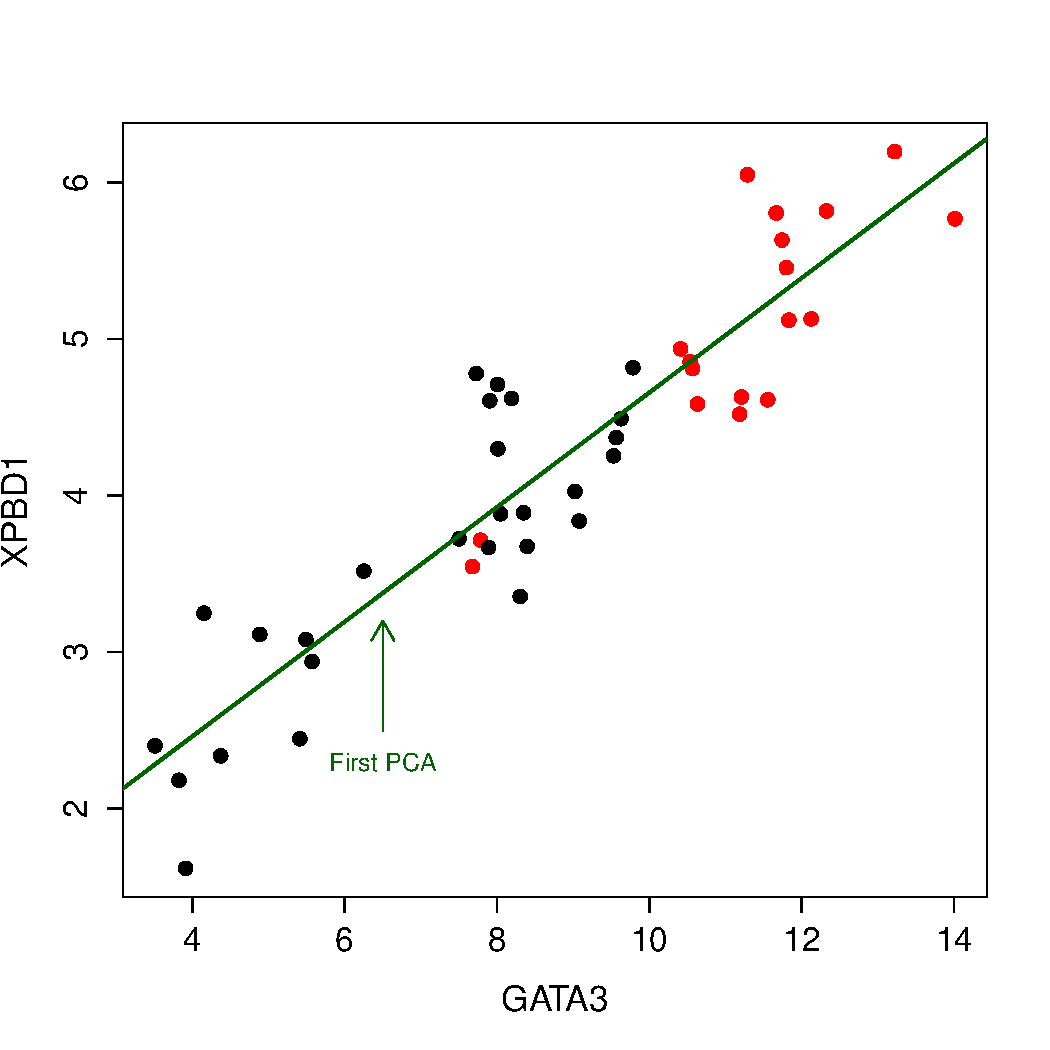
\includegraphics[width=2in]{figure/plot_pca_2-1} 

}



\end{knitrout}

\end{frame}


\begin{frame}[fragile, plain]\frametitle{Principal component analysis}

\begin{knitrout}\footnotesize
\definecolor{shadecolor}{rgb}{0.969, 0.969, 0.969}\color{fgcolor}

{\centering 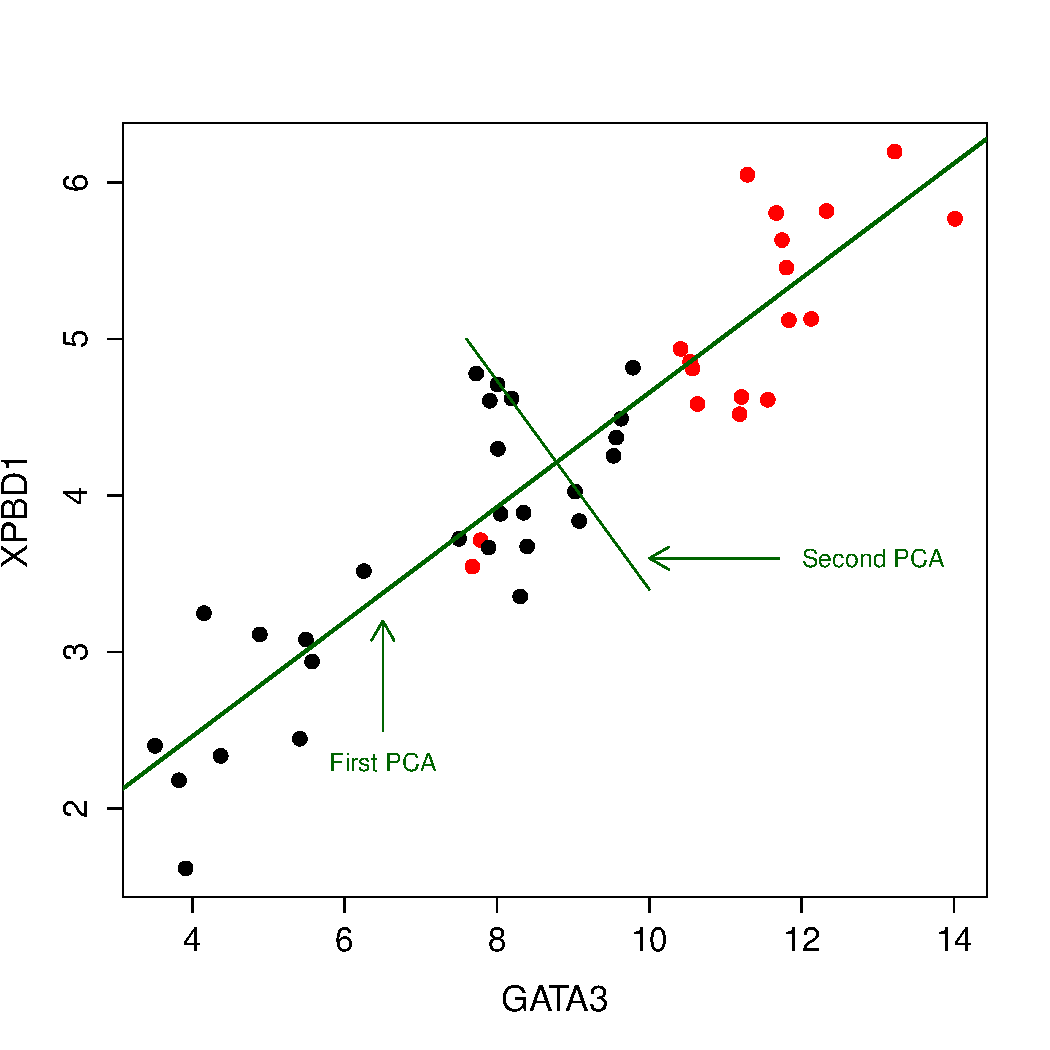
\includegraphics[width=2in]{figure/plot_pca_3-1} 

}



\end{knitrout}

\end{frame}




\begin{frame}[plain]{Principal component analysis}

\begin{itemize} 
 \item Correlations between variables and the principal axes are known as \textbf{loadings}
 \item Each element represents the contribution of a given variable to a component (\textbf{eigenvalues})
\end{itemize}

\end{frame}

\begin{frame}[plain]{Principal component analysis}

 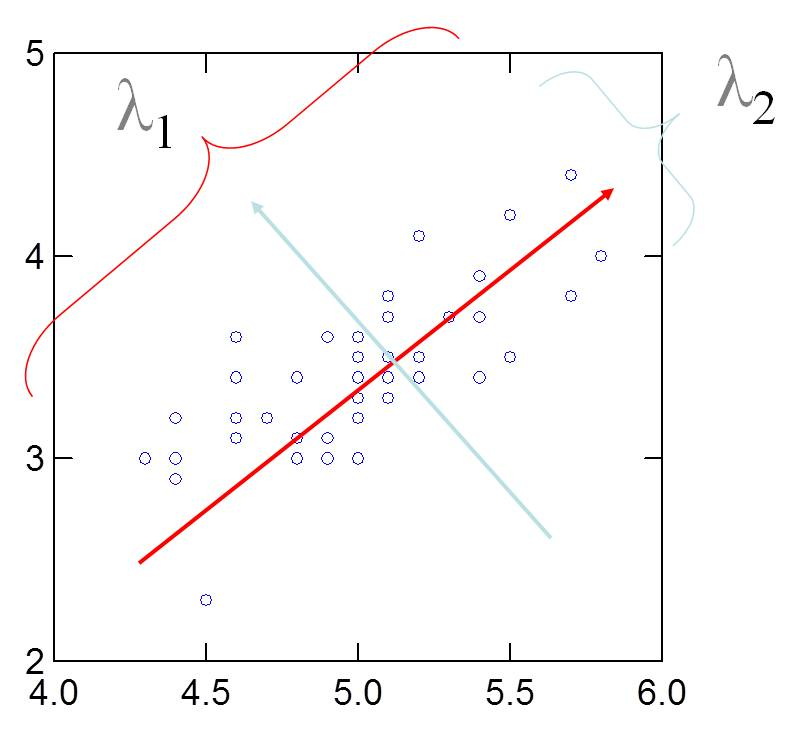
\includegraphics[height=4.5cm, width=4.5cm]{figures/pca2.jpg}
 
\end{frame}


\begin{frame}[plain]{PCA: How many axes are needed?}

\begin{itemize}
 \item Does the $(k+1)^{th}$ principal axis represent more variance that would e expected by chance?
 \item Several tests and rules have been proposed (\textbf{Horn\'s method} and bootstrap approach)
 \item A common \emph{rule of thumb}, when PCA is based on correlations, is that axes with eigenvalues $> 1$ are worth interpreting
\end{itemize}
\end{frame}

\begin{frame}[plain]{PCA: non-linear relationships}

\begin{itemize}
 \item PCA assumes relationships among variables are LINEAR
 \item If the sctructure in the data is NONLINEAR (the cloud of points twists and curves its way through $p$-dimensional space) the principal axes will not be an efficient and informative summary of the data
 \item Use Principal Curve Analysis
\end{itemize}
\end{frame}

\begin{frame}[fragile, plain]{Principal components analysis with R}

\begin{knitrout}\footnotesize
\definecolor{shadecolor}{rgb}{0.969, 0.969, 0.969}\color{fgcolor}\begin{kframe}
\begin{alltt}
\hlkwd{require}\hlstd{(graphics)}
\hlkwd{data}\hlstd{(USArrests)}
\hlkwd{head}\hlstd{(USArrests)}
\end{alltt}
\begin{verbatim}
##            Murder Assault UrbanPop Rape
## Alabama      13.2     236       58 21.2
## Alaska       10.0     263       48 44.5
## Arizona       8.1     294       80 31.0
## Arkansas      8.8     190       50 19.5
## California    9.0     276       91 40.6
## Colorado      7.9     204       78 38.7
\end{verbatim}
\end{kframe}
\end{knitrout}
\end{frame}


\begin{frame}[fragile, plain]{Principal components analysis with R}

\begin{knitrout}\footnotesize
\definecolor{shadecolor}{rgb}{0.969, 0.969, 0.969}\color{fgcolor}\begin{kframe}
\begin{alltt}
\hlkwd{princomp}\hlstd{(USArrests)}
\end{alltt}
\begin{verbatim}
## Call:
## princomp(x = USArrests)
## 
## Standard deviations:
##    Comp.1    Comp.2    Comp.3    Comp.4 
## 82.890847 14.069560  6.424204  2.457837 
## 
##  4  variables and  50 observations.
\end{verbatim}
\begin{alltt}
\hlstd{mod} \hlkwb{<-} \hlkwd{princomp}\hlstd{(USArrests)}
\hlkwd{summary}\hlstd{(mod)}
\end{alltt}
\begin{verbatim}
## Importance of components:
##                            Comp.1      Comp.2      Comp.3       Comp.4
## Standard deviation     82.8908472 14.06956001 6.424204055 2.4578367034
## Proportion of Variance  0.9655342  0.02781734 0.005799535 0.0008489079
## Cumulative Proportion   0.9655342  0.99335156 0.999151092 1.0000000000
\end{verbatim}
\end{kframe}
\end{knitrout}
\end{frame}


\begin{frame}[fragile, plain]{Principal components analysis with R}

\begin{knitrout}\footnotesize
\definecolor{shadecolor}{rgb}{0.969, 0.969, 0.969}\color{fgcolor}\begin{kframe}
\begin{alltt}
\hlstd{mod2} \hlkwb{<-} \hlkwd{princomp}\hlstd{(USArrests)}
\hlkwd{summary}\hlstd{(mod2)}
\end{alltt}
\begin{verbatim}
## Importance of components:
##                            Comp.1      Comp.2      Comp.3       Comp.4
## Standard deviation     82.8908472 14.06956001 6.424204055 2.4578367034
## Proportion of Variance  0.9655342  0.02781734 0.005799535 0.0008489079
## Cumulative Proportion   0.9655342  0.99335156 0.999151092 1.0000000000
\end{verbatim}
\end{kframe}
\end{knitrout}
\end{frame}

\begin{frame}[fragile, plain]{Principal components analysis with R}
\begin{knitrout}\footnotesize
\definecolor{shadecolor}{rgb}{0.969, 0.969, 0.969}\color{fgcolor}\begin{kframe}
\begin{alltt}
\hlkwd{plot}\hlstd{(mod2)}
\end{alltt}
\end{kframe}

{\centering 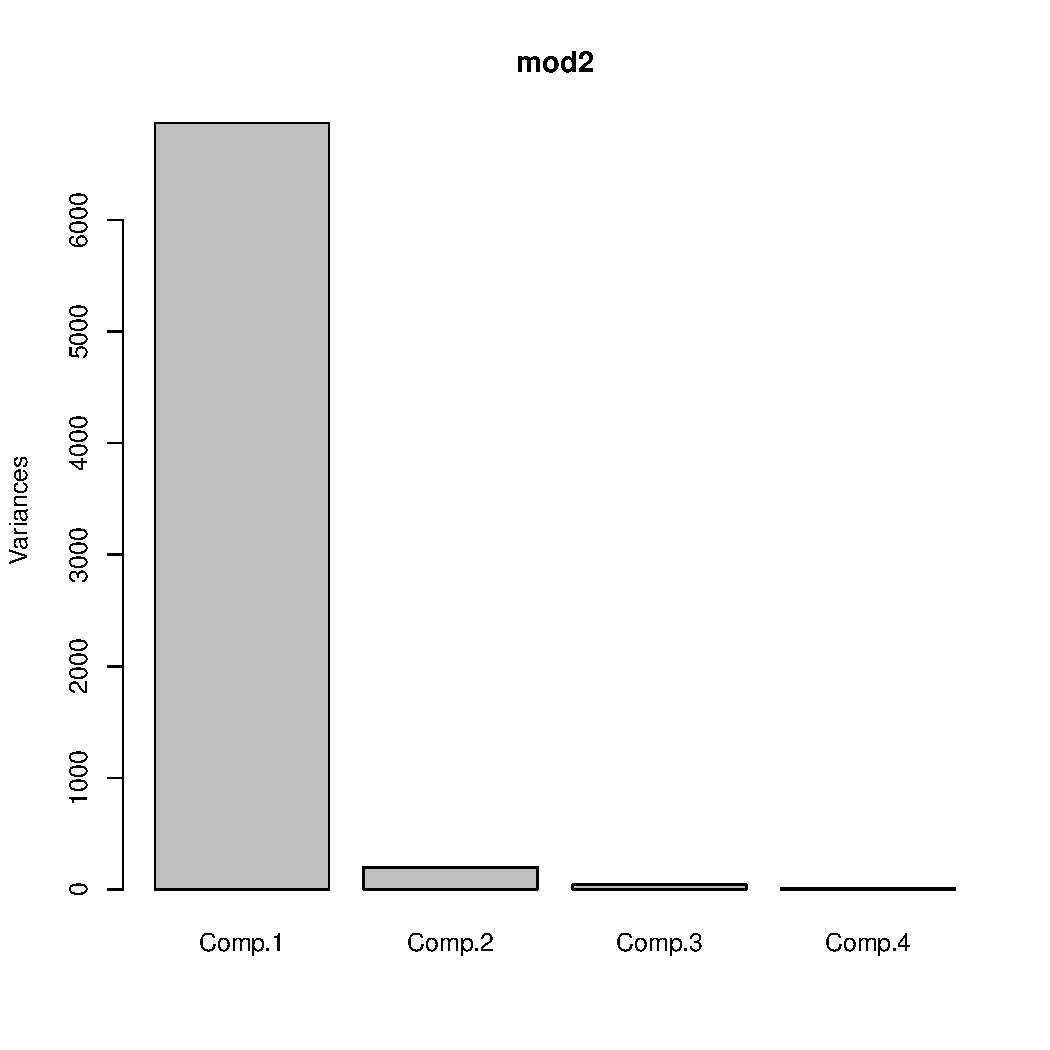
\includegraphics[width=2in]{figure/plotPCA-1} 

}



\end{knitrout}
\end{frame}


\begin{frame}[fragile, plain]{Principal components analysis with R}
\noindent Help interpreting the results
\begin{knitrout}\footnotesize
\definecolor{shadecolor}{rgb}{0.969, 0.969, 0.969}\color{fgcolor}\begin{kframe}
\begin{alltt}
\hlkwd{loadings}\hlstd{(mod2)}
\end{alltt}
\begin{verbatim}
## 
## Loadings:
##          Comp.1 Comp.2 Comp.3 Comp.4
## Murder                         0.995
## Assault   0.995                     
## UrbanPop        -0.977 -0.201       
## Rape            -0.201  0.974       
## 
##                Comp.1 Comp.2 Comp.3 Comp.4
## SS loadings      1.00   1.00   1.00   1.00
## Proportion Var   0.25   0.25   0.25   0.25
## Cumulative Var   0.25   0.50   0.75   1.00
\end{verbatim}
\end{kframe}
\end{knitrout}
\end{frame}


\begin{frame}[fragile, plain]{Principal components analysis with R}

\begin{knitrout}\footnotesize
\definecolor{shadecolor}{rgb}{0.969, 0.969, 0.969}\color{fgcolor}\begin{kframe}
\begin{alltt}
\hlkwd{biplot}\hlstd{(mod2)}
\end{alltt}
\end{kframe}

{\centering 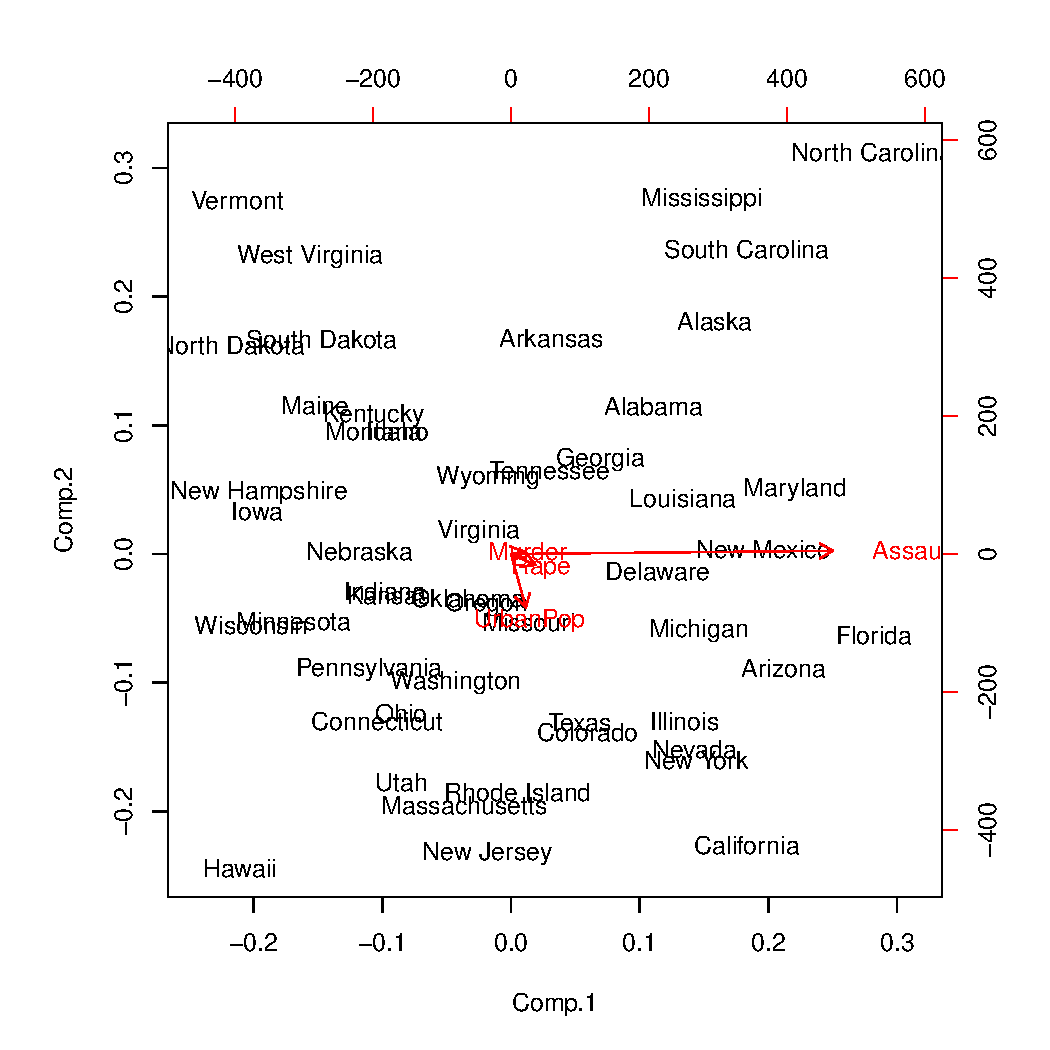
\includegraphics[width=2in]{figure/pcaPlot3-1} 

}



\end{knitrout}
\end{frame}


\begin{frame}[fragile, plain]{PCA improving visualization}

\begin{itemize}
  \item Data from the Cancer Genome Atlas (TCGA) will be analyzed.
  \item A subset of the TCGA breast cancer study from Nature 2012 publication have been selected.
  \item Data {\tt https://tcga-data.nci.nih.gov/docs/publications/brca\_2012/}.
  \item Available data are: miRNA, miRNAprecursor, RNAseq, Methylation, proteins from a RPPA array, and  GISTIC SNP calls (CNA and LOH). Clinical data are also available.
  \item We are interested in comparing women with ER+ vs ER-.
 \end{itemize}
 
\end{frame}


\begin{frame}[fragile, plain]{PCA improving visualization}

\begin{knitrout}\footnotesize
\definecolor{shadecolor}{rgb}{0.969, 0.969, 0.969}\color{fgcolor}\begin{kframe}
\begin{alltt}
\hlkwd{library}\hlstd{(made4)}
\hlkwd{load}\hlstd{(}\hlstr{"data/breast_TCGA.RData"}\hlstd{)}
\hlstd{group} \hlkwb{<-} \hlkwd{droplevels}\hlstd{(breast_multi}\hlopt{$}\hlstd{clin}\hlopt{$}\hlstd{ER.Status)}
\hlstd{rnaseq} \hlkwb{<-} \hlstd{breast_multi}\hlopt{$}\hlstd{RNAseq}
\hlstd{out} \hlkwb{<-} \hlkwd{ord}\hlstd{(rnaseq,} \hlkwc{trans}\hlstd{=}\hlnum{FALSE}\hlstd{,} \hlkwc{type}\hlstd{=}\hlstr{"pca"}\hlstd{,} \hlkwc{classvec}\hlstd{=group)}
\hlkwd{plot}\hlstd{(out,} \hlkwc{nlab}\hlstd{=}\hlnum{3}\hlstd{,} \hlkwc{arraylabels}\hlstd{=}\hlkwd{rep}\hlstd{(}\hlstr{"T"}\hlstd{,} \hlnum{79}\hlstd{))}
\end{alltt}
\end{kframe}

{\centering 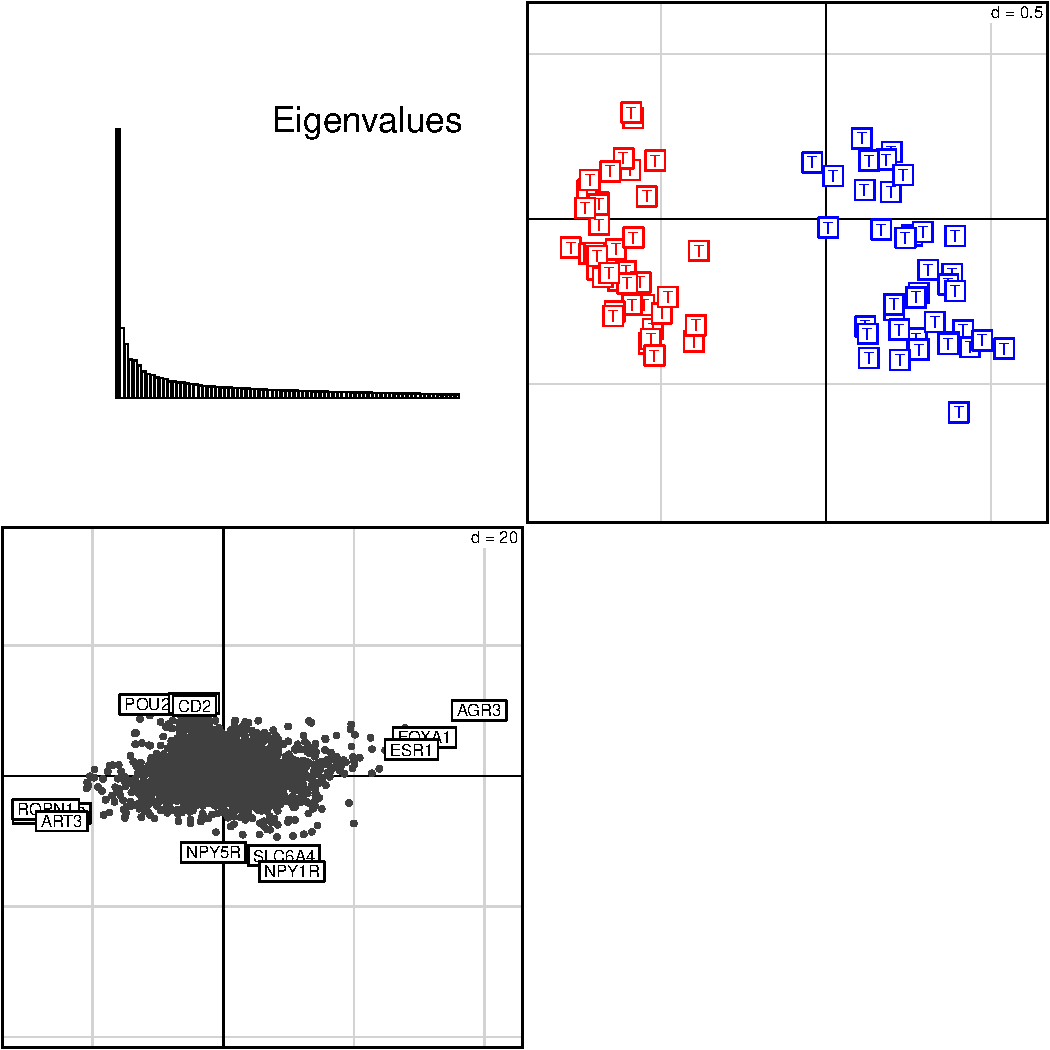
\includegraphics[width=2in]{figure/plotPCA2-1} 

}



\end{knitrout}
\end{frame}


\begin{frame}[fragile, plain]{PCA improving visualization}

\begin{knitrout}\footnotesize
\definecolor{shadecolor}{rgb}{0.969, 0.969, 0.969}\color{fgcolor}\begin{kframe}
\begin{alltt}
\hlkwd{par}\hlstd{(}\hlkwc{mfrow}\hlstd{=}\hlkwd{c}\hlstd{(}\hlnum{2}\hlstd{,}\hlnum{1}\hlstd{))}
\hlkwd{plotarrays}\hlstd{(out}\hlopt{$}\hlstd{ord}\hlopt{$}\hlstd{co,} \hlkwc{classvec}\hlstd{=group)}
\hlkwd{plotgenes}\hlstd{(out,} \hlkwc{col}\hlstd{=}\hlstr{"blue"}\hlstd{)}
\end{alltt}
\end{kframe}

{\centering 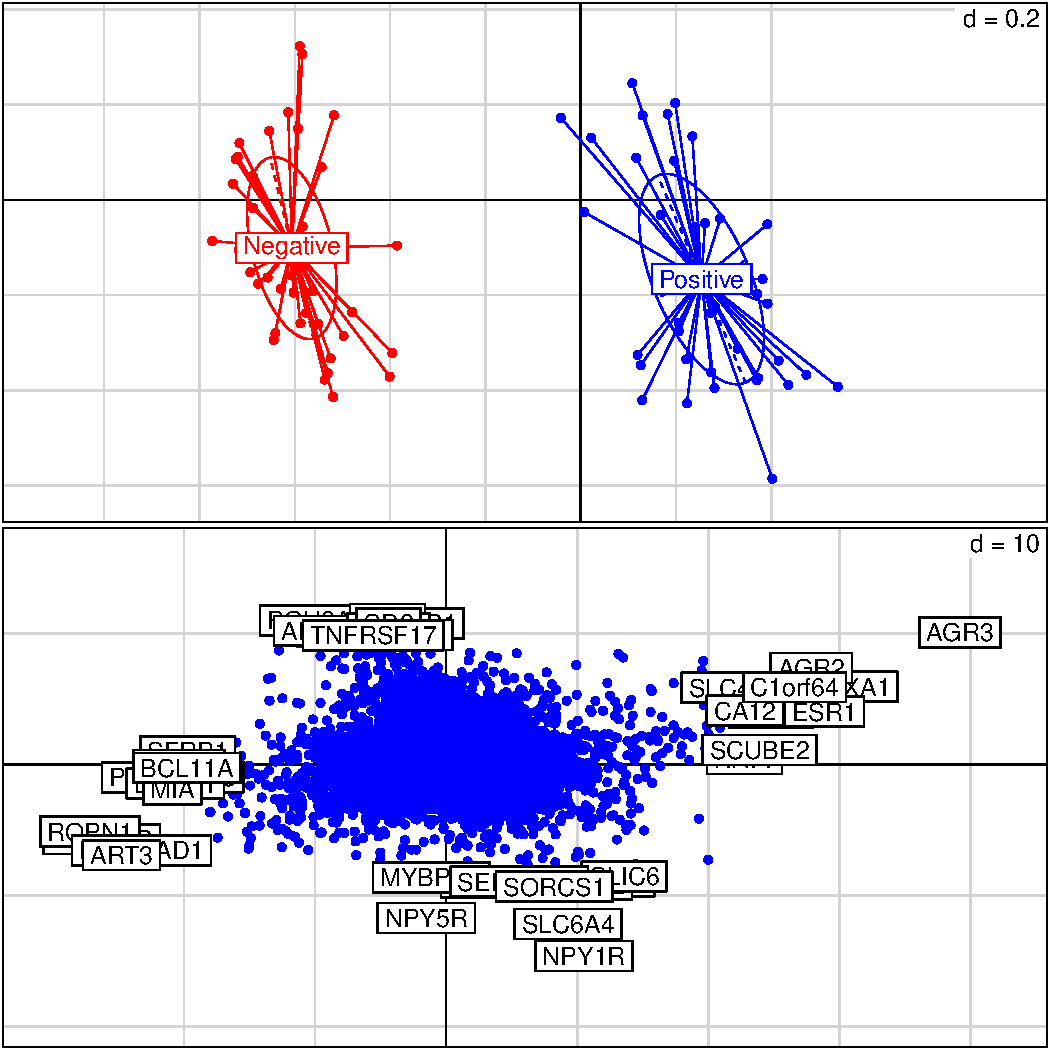
\includegraphics[width=2in]{figure/plotPCA2b-1} 

}



\end{knitrout}

\end{frame}

\begin{frame}[fragile, plain]{PCA improving visualization}

A list of variables with higher loadings on axes can be obtained using the following
function

\begin{knitrout}\footnotesize
\definecolor{shadecolor}{rgb}{0.969, 0.969, 0.969}\color{fgcolor}\begin{kframe}
\begin{alltt}
\hlstd{ax1} \hlkwb{<-} \hlkwd{topgenes}\hlstd{(out,} \hlkwc{axis}\hlstd{=}\hlnum{1}\hlstd{,} \hlkwc{n}\hlstd{=}\hlnum{5}\hlstd{,} \hlkwc{ends}\hlstd{=}\hlstr{"pos"}\hlstd{)}
\hlstd{ax2} \hlkwb{<-} \hlkwd{topgenes}\hlstd{(out,} \hlkwc{axis}\hlstd{=}\hlnum{2}\hlstd{,} \hlkwc{n}\hlstd{=}\hlnum{5}\hlstd{,} \hlkwc{ends}\hlstd{=}\hlstr{"neg"}\hlstd{)}
\hlkwd{cbind}\hlstd{(}\hlkwc{pos}\hlstd{=ax1,} \hlkwc{neg}\hlstd{=ax2)}
\end{alltt}
\begin{verbatim}
##      pos       neg     
## [1,] "AGR3"    "NPY1R" 
## [2,] "FOXA1"   "SLC6A4"
## [3,] "ESR1"    "NPY5R" 
## [4,] "AGR2"    "SORCS1"
## [5,] "C1orf64" "CST9L"
\end{verbatim}
\end{kframe}
\end{knitrout}

\end{frame}


%%%%%%%%%%%%%%%%%%%%%%%%%%%%%%%%%%%%%%%%%
\subsection{PCA requirements}
%%%%%%%%%%%%%%%%%%%%%%%%%%%%%%%%%%%%%%%%%



\begin{frame}[fragile, plain]{PCA requirements}

\begin{itemize}
  \item Data scale
\begin{knitrout}\footnotesize
\definecolor{shadecolor}{rgb}{0.969, 0.969, 0.969}\color{fgcolor}\begin{kframe}
\begin{alltt}
  \hlstd{rnaseq.s} \hlkwb{<-} \hlkwd{scale}\hlstd{(rnaseq,} \hlkwc{center}\hlstd{=} \hlnum{TRUE}\hlstd{,} \hlkwc{scale} \hlstd{=} \hlnum{TRUE}\hlstd{)}
\end{alltt}
\end{kframe}
\end{knitrout}
 \item Complete cases
\begin{knitrout}\footnotesize
\definecolor{shadecolor}{rgb}{0.969, 0.969, 0.969}\color{fgcolor}\begin{kframe}
\begin{alltt}
\hlkwd{library}\hlstd{(impute)}
\hlstd{rnaseq.s.imp} \hlkwb{<-} \hlkwd{impute.knn}\hlstd{(rnaseq.s,} \hlkwc{rowmax} \hlstd{=} \hlnum{0.5}\hlstd{,}
                         \hlkwc{colmax} \hlstd{=} \hlnum{0.8}\hlstd{)}\hlopt{$}\hlstd{data} \hlcom{#samples in columns!!!}
\end{alltt}
\begin{verbatim}
## Cluster size 10020 broken into 1909 8111 
## Cluster size 1909 broken into 325 1584 
## Done cluster 325 
## Cluster size 1584 broken into 1498 86 
## Done cluster 1498 
## Done cluster 86 
## Done cluster 1584 
## Done cluster 1909 
## Cluster size 8111 broken into 5038 3073 
## Cluster size 5038 broken into 1351 3687 
## Done cluster 1351 
## Cluster size 3687 broken into 1738 1949 
## Cluster size 1738 broken into 768 970 
## Done cluster 768 
## Done cluster 970 
## Done cluster 1738 
## Cluster size 1949 broken into 981 968 
## Done cluster 981 
## Done cluster 968 
## Done cluster 1949 
## Done cluster 3687 
## Done cluster 5038 
## Cluster size 3073 broken into 747 2326 
## Done cluster 747 
## Cluster size 2326 broken into 1984 342 
## Cluster size 1984 broken into 456 1528 
## Done cluster 456 
## Cluster size 1528 broken into 954 574 
## Done cluster 954 
## Done cluster 574 
## Done cluster 1528 
## Done cluster 1984 
## Done cluster 342 
## Done cluster 2326 
## Done cluster 3073 
## Done cluster 8111
\end{verbatim}
\end{kframe}
\end{knitrout}
\end{itemize}
\end{frame}


\begin{frame}[fragile, plain]{PCA requirements}
\begin{knitrout}\footnotesize
\definecolor{shadecolor}{rgb}{0.969, 0.969, 0.969}\color{fgcolor}\begin{kframe}
\begin{alltt}
\hlstd{out} \hlkwb{<-} \hlkwd{ord}\hlstd{(rnaseq.s.imp,} \hlkwc{trans}\hlstd{=}\hlnum{FALSE}\hlstd{,} \hlkwc{type}\hlstd{=}\hlstr{"pca"}\hlstd{,} \hlkwc{classvec}\hlstd{=group)}
\hlkwd{plot}\hlstd{(out,} \hlkwc{nlab}\hlstd{=}\hlnum{3}\hlstd{,} \hlkwc{arraylabels}\hlstd{=}\hlkwd{rep}\hlstd{(}\hlstr{"T"}\hlstd{,} \hlnum{79}\hlstd{))}
\end{alltt}
\end{kframe}

{\centering 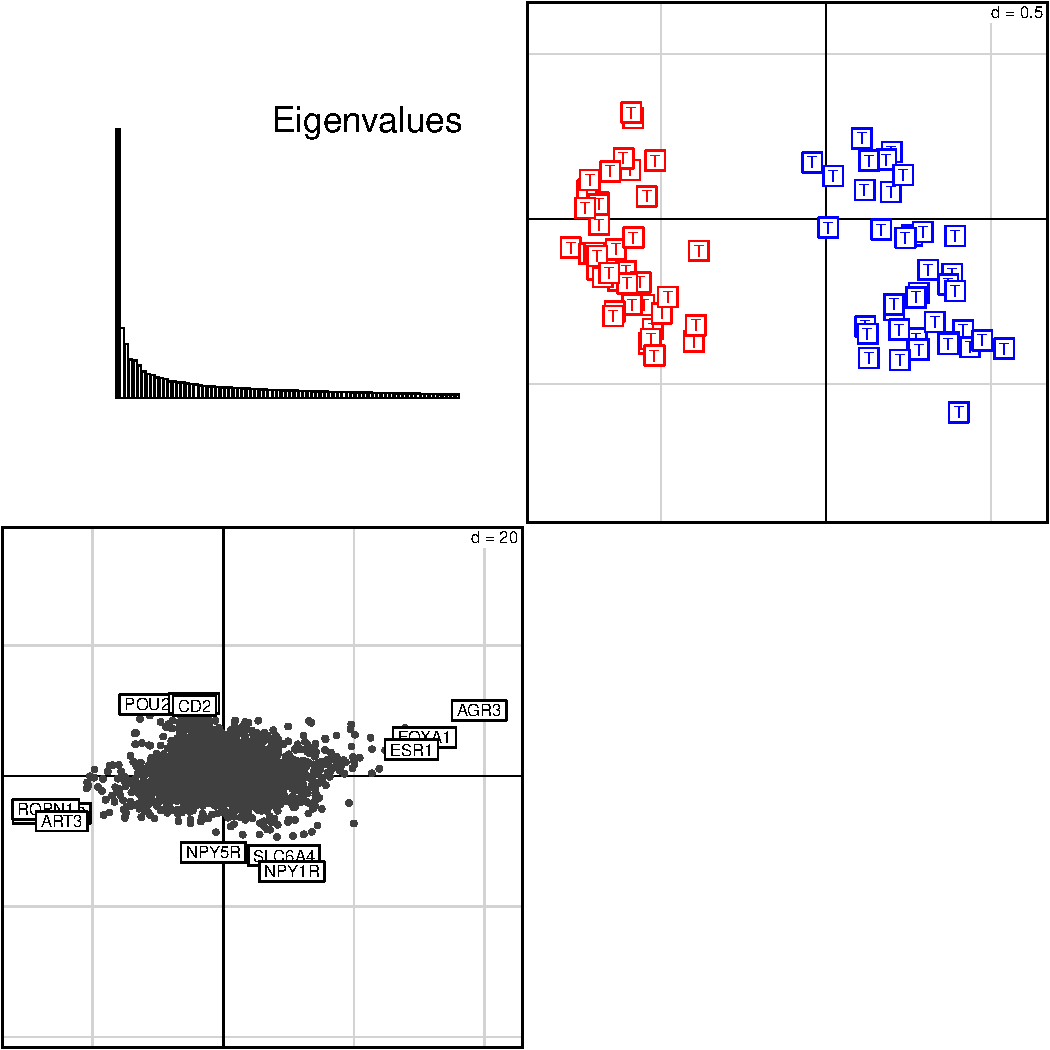
\includegraphics[width=2in]{figure/plotPCA3-1} 

}



\end{knitrout}
\end{frame}

\begin{frame}[fragile, plain]{Variance explained}
\begin{knitrout}\footnotesize
\definecolor{shadecolor}{rgb}{0.969, 0.969, 0.969}\color{fgcolor}\begin{kframe}
\begin{alltt}
\hlkwd{summary}\hlstd{(out}\hlopt{$}\hlstd{ord)}
\end{alltt}
\begin{verbatim}
## Class: pca dudi
## Call: dudi.pca(df = data.tr, scannf = FALSE, nf = ord.nf)
## 
## Total inertia: 79
## 
## Eigenvalues:
##     Ax1     Ax2     Ax3     Ax4     Ax5 
##  18.526   4.817   3.709   2.640   2.591 
## 
## Projected inertia (%):
##     Ax1     Ax2     Ax3     Ax4     Ax5 
##  23.450   6.097   4.695   3.342   3.279 
## 
## Cumulative projected inertia (%):
##     Ax1   Ax1:2   Ax1:3   Ax1:4   Ax1:5 
##   23.45   29.55   34.24   37.58   40.86 
## 
## (Only 5 dimensions (out of 79) are shown)
\end{verbatim}
\end{kframe}
\end{knitrout}
\end{frame}


%%%%%%%%%%%%%%%%%%%%%%%%%%%%%%%%%%%%%%%%%
\subsection{Number of significant components}
%%%%%%%%%%%%%%%%%%%%%%%%%%%%%%%%%%%%%%%%%


\begin{frame}[fragile, plain]{PCA number of significant components}

\begin{itemize}
 \item  Parallel analysis (Horn) \url{http://files.eric.ed.gov/fulltext/EJ1101205.pdf}
 \item Bootstrap method (Eigenvalues)
\end{itemize}

\begin{knitrout}\footnotesize
\definecolor{shadecolor}{rgb}{0.969, 0.969, 0.969}\color{fgcolor}\begin{kframe}
\begin{alltt}
\hlkwd{library}\hlstd{(nFactors)}
\hlstd{ev} \hlkwb{<-} \hlkwd{eigen}\hlstd{(}\hlkwd{cor}\hlstd{(USArrests))} \hlcom{# get eigenvalues}
\hlstd{ap} \hlkwb{<-} \hlkwd{parallel}\hlstd{(}\hlkwc{subject}\hlstd{=}\hlkwd{nrow}\hlstd{(USArrests),} \hlkwc{var}\hlstd{=}\hlkwd{ncol}\hlstd{(USArrests),}
  \hlkwc{rep}\hlstd{=}\hlnum{100}\hlstd{,}\hlkwc{cent}\hlstd{=}\hlnum{.05}\hlstd{)}
\hlstd{nS} \hlkwb{<-} \hlkwd{nScree}\hlstd{(}\hlkwc{x}\hlstd{=ev}\hlopt{$}\hlstd{values,} \hlkwc{aparallel}\hlstd{=ap}\hlopt{$}\hlstd{eigen}\hlopt{$}\hlstd{qevpea)}
\hlkwd{plotnScree}\hlstd{(nS)}
\end{alltt}
\end{kframe}
\end{knitrout}
\end{frame}


\begin{frame}[plain]{PCA number of significant components}

 \begin{figure}
 \begin{center}
   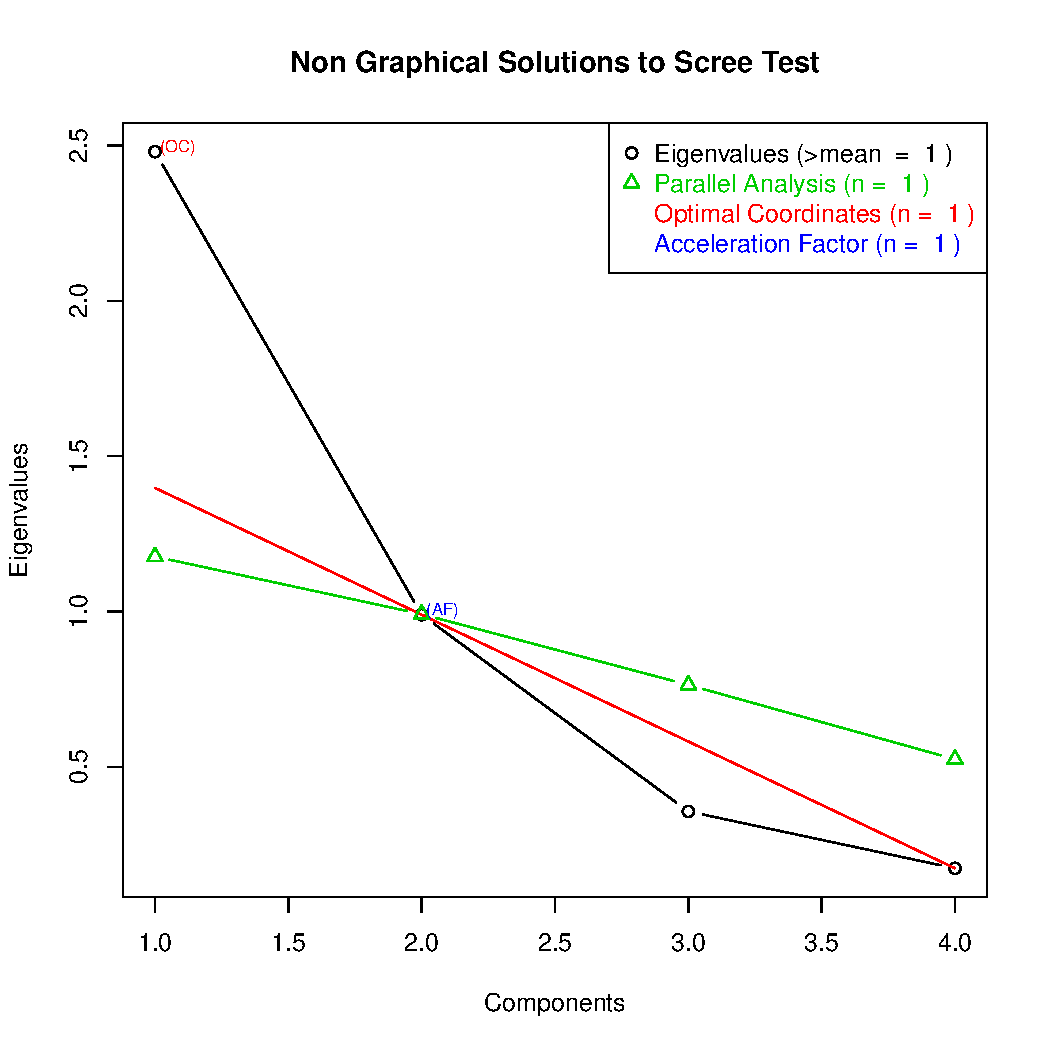
\includegraphics[height=5cm, width=5cm]{figure/boot-1}
 \end{center}

\end{figure}\end{frame}


%%%%%%%%%%%%%%%%%%%%%%%%%%%%%%%%%%%%%%%%%
\subsection{Principal curves}
%%%%%%%%%%%%%%%%%%%%%%%%%%%%%%%%%%%%%%%%%


\begin{frame}{Principal curves}

 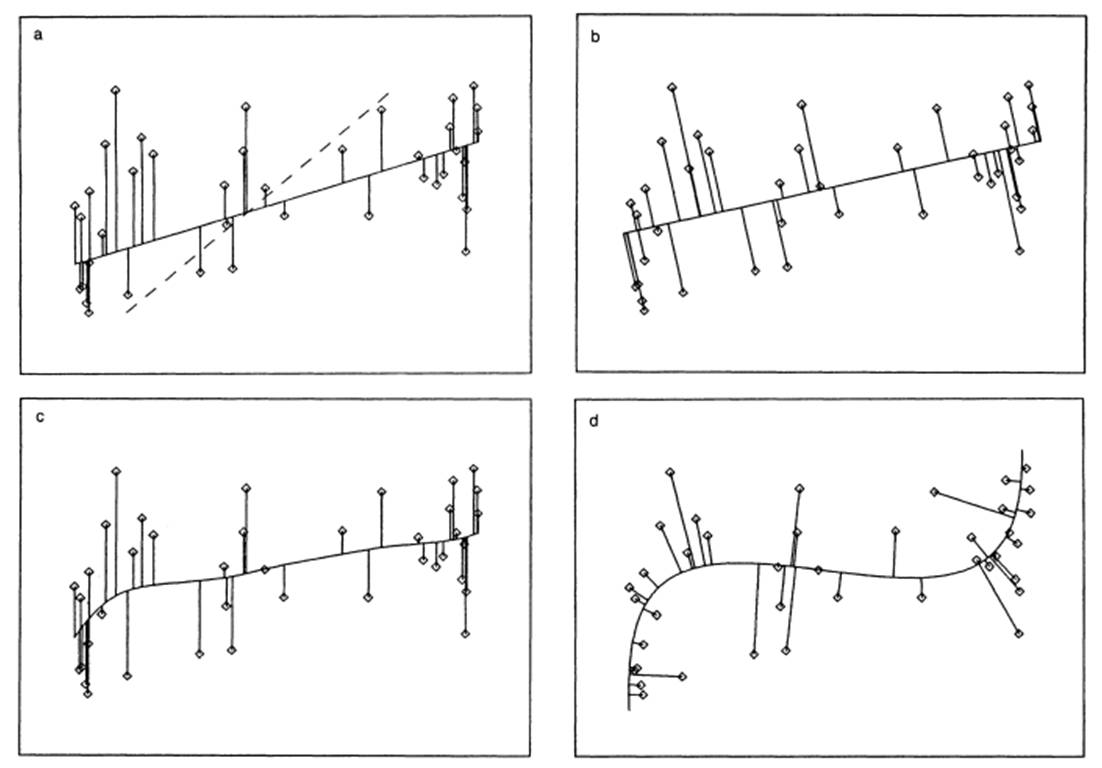
\includegraphics{figures/pcurve.jpg}
 
\end{frame}


\begin{frame}[fragile, plain]{Principal curves}
\noindent \textbf{Example:}  Spectral decomposition of stellar objects, generated in the framework of the Gaia project.
\begin{knitrout}\footnotesize
\definecolor{shadecolor}{rgb}{0.969, 0.969, 0.969}\color{fgcolor}\begin{kframe}
\begin{alltt}
\hlkwd{require}\hlstd{(LPCM)}
\hlkwd{data}\hlstd{(gaia)}
\hlkwd{dim}\hlstd{(gaia)}
\end{alltt}
\begin{verbatim}
## [1] 8286   20
\end{verbatim}
\begin{alltt}
\hlkwd{names}\hlstd{(gaia)}
\end{alltt}
\begin{verbatim}
##  [1] "ID"          "metallicity" "gravity"     "temperature" "band1"      
##  [6] "band2"       "band3"       "band4"       "band5"       "band6"      
## [11] "band7"       "band8"       "band9"       "band10"      "band11"     
## [16] "band12"      "band13"      "band14"      "band15"      "band16"
\end{verbatim}
\end{kframe}
\end{knitrout}
\end{frame}


\begin{frame}[fragile, plain]{Principal curves}

\begin{knitrout}\footnotesize
\definecolor{shadecolor}{rgb}{0.969, 0.969, 0.969}\color{fgcolor}\begin{kframe}
\begin{alltt}
 \hlstd{lpc1} \hlkwb{<-}  \hlkwd{lpc}\hlstd{(gaia[,}\hlnum{7}\hlopt{:}\hlnum{8}\hlstd{])}
 \hlkwd{plot}\hlstd{(lpc1,} \hlkwc{curvecol}\hlstd{=}\hlstr{"red"}\hlstd{,} \hlkwc{lwd}\hlstd{=}\hlnum{3}\hlstd{)}
\end{alltt}
\end{kframe}

{\centering 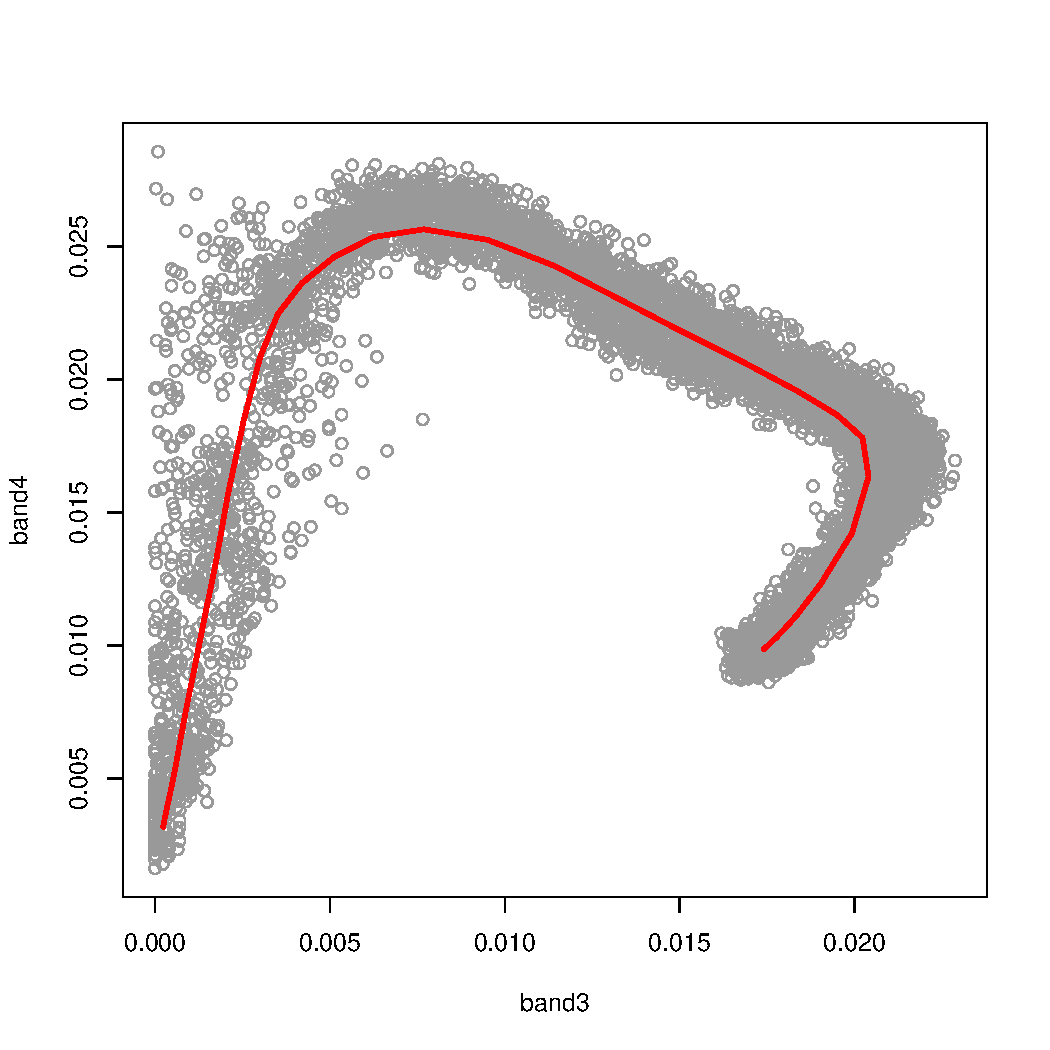
\includegraphics[width=2in]{figure/lcpmPlot-1} 

}



\end{knitrout}

\end{frame}

\begin{frame}[fragile, plain]{Principal curves}

\begin{knitrout}\footnotesize
\definecolor{shadecolor}{rgb}{0.969, 0.969, 0.969}\color{fgcolor}\begin{kframe}
\begin{alltt}
\hlkwd{require}\hlstd{(scatterplot3d)}
\hlstd{lpc2} \hlkwb{<-} \hlkwd{lpc}\hlstd{(gaia[,}\hlnum{7}\hlopt{:}\hlnum{9}\hlstd{])}
\hlkwd{plot}\hlstd{(lpc2,} \hlkwc{curvecol}\hlstd{=}\hlnum{2}\hlstd{,} \hlkwc{type}\hlstd{=}\hlkwd{c}\hlstd{(}\hlstr{"curve"}\hlstd{,}\hlstr{"mass"}\hlstd{))}
\end{alltt}
\end{kframe}

{\centering 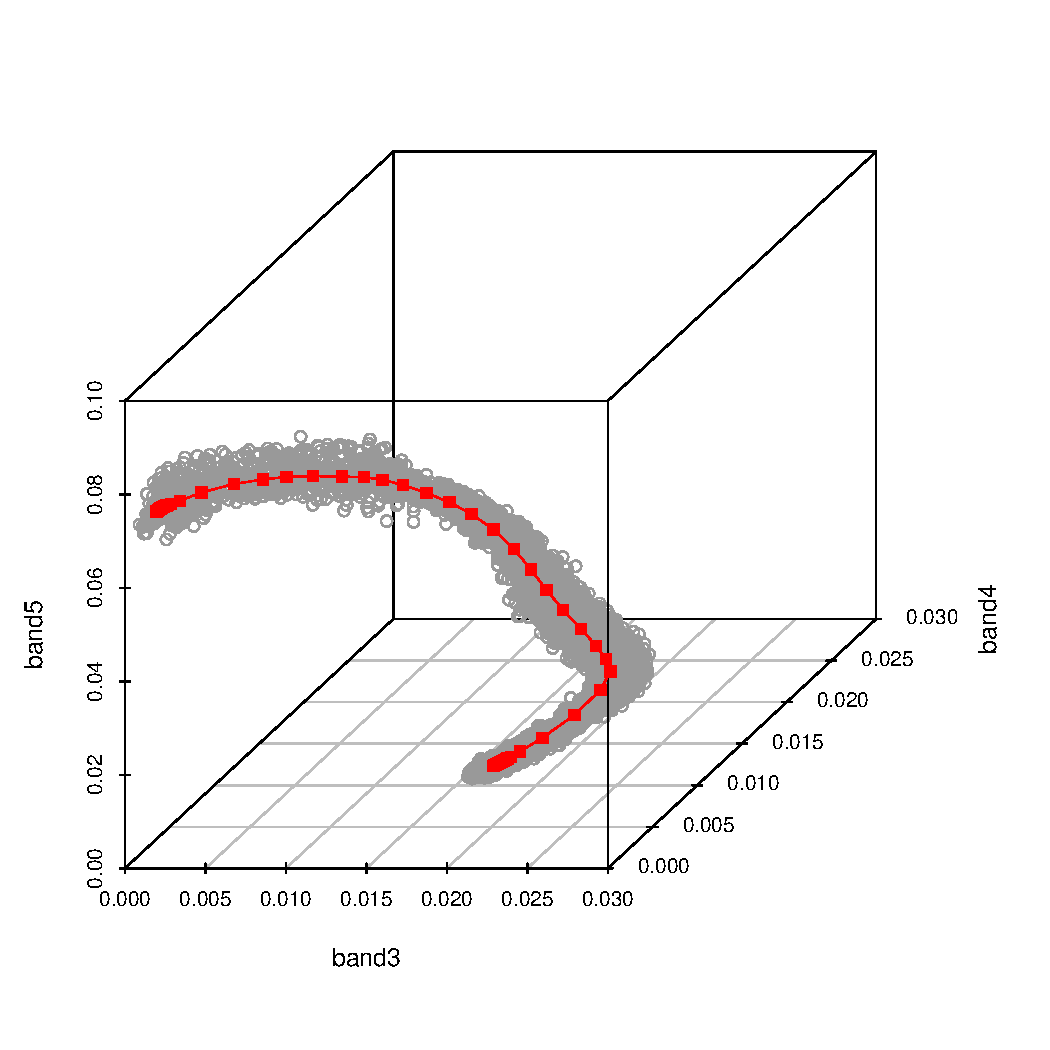
\includegraphics[width=2in]{figure/lcpmPlot2-1} 

}



\end{knitrout}

\end{frame}



%%%%%%%%%%%%%%%%%%%%%%%%%%%%%%%%%%%%%%%%%
\subsection{Improvements of PCA}
%%%%%%%%%%%%%%%%%%%%%%%%%%%%%%%%%%%%%%%%%


\begin{frame}[fragile, plain]\frametitle{Improvements of PCA}

\begin{itemize}
\item There are other thechniques such as: Principal co-ordinate analysis (PCoA) or Multidimensional scaling (MDS), correspondence analysis (CA) and nonsymetrical correspondence analysis (NSCA).
\pause
\item They can be applied to other types of data (e.g. non-continuous). PCoA can also be applied to binary or count data.
\pause
\item PCA is designed to analyze multi-normal distributed data. If data are skweed, contain extreme outliers, or display nonlinear trends, other methods such as 
PCoA or MDS should be used instead.
\pause
\item Nonnegative matrix factorization (NMF) and Independent Component Analysis (ICA) are applied when orthogonality or independence acrross components are not hold.
\end{itemize}

\end{frame}


\begin{frame}[fragile, plain]\frametitle{Improvements of PCA}

\begin{itemize}
\item Solving the problem for the $i$-th component $$ \argmax_{q^i} \text{var}(Xq^i)$$ uses SVD decomposition and it requires and inversion step that can be problematic when   $p >> n$
\item Several extensions based on reguralization step or L-1 penalization (Least Absolute Shrinkage and Selection Operator, LASSO) can be applied
\item Sparse, penalized and reguralized extensions of PCA and related method have been recently proposed in omic data analysis.
\end{itemize}
\end{frame}


\begin{frame}[plain]\frametitle{Multidimensional scalling}

\begin{itemize}
\item PCA requires (multivariate) data normallity. This is an strong assumption.
\item Multidimensional scalling (MDS) creates a plot displaying the relative positions of a number of 
variables, given only a table of the distances between them.
\item There are two main methods for solving MDS
\begin{enumerate}
\item Classical Multidimensional Scaling reproduces the original metric or distances. 
\item Non-Metric Multidimensional Scaling assumes that only the ranks of the distances are known. Hence, this method produces a map which tries to reproduce these ranks. 
\item  MDS can be performed using {\tt cmdscale} function.
 \end{enumerate}
\end{itemize}
\end{frame}





%%%%%%%%%%%%%%%%%%%%%%%%%%%%%%%%%%%
\section{Clustering methods}
%%%%%%%%%%%%%%%%%%%%%%%%%%%%%%%%%%%


\begin{frame}[fragile, plain]{Clustering methods}

\begin{itemize}
 \item The goal is to group samples (rows) or features (columns) or both (bi-Clustering)
  according to how separated are the groups.
 \item This 'separation' is measure using a \textbf{dissimilarity measure}
 \item Classes of each individual/feature is not know
 \item Therefore, it is known as non-supervised Clustering  
\end{itemize}

\end{frame}


\begin{frame}[fragile, plain]{Clustering methods}

\begin{itemize}
 \item A good clustering method will produce hihg quality clusters with
   \begin{itemize}
    \item High intra-class similarity
    \item low inter-class similarity
   \end{itemize} 
 \item The quality of a clustering result depends on both the similarity measure used
       by the method and its implementation
 \item The quality of a clustering method is also measured by its ability to dicover hidden patterns
      
\end{itemize}

\end{frame}



\begin{frame}[fragile, plain]{Clustering methods}

\begin{itemize}
 \item \textbf{Hierarchical algorithms}: Create a hierarchical decomposition
        (agglomerative o divisive) of the set of data using some criterion
 \item \textbf{Partitioning algorithms}: Construct several partitions and the evaluate them by some
        criterion 
     \begin{itemize}
       \item k-means: each cluster is represented by the center of the cluster
       \item k-medoids (or PAM): each cluster is represented by one of the objects in the cluster
     \end{itemize}
 \item \textbf{Model-based}: A model is hypothesized for each of the clusters and the idea is to find
        the best fit of the data given the model
      
\end{itemize}

\end{frame}


%%%%%%%%%%%%%%%%%%%%%%%%%%%%%%%%%%%
\subsection{Hierarchical clustering}
%%%%%%%%%%%%%%%%%%%%%%%%%%%%%%%%%%%

\begin{frame}[fragile, plain]{Hierarchical clustering}
Use distance matrix as clustering criteria. This method does not require the number of clusters, but needs a termination condition.

\medskip

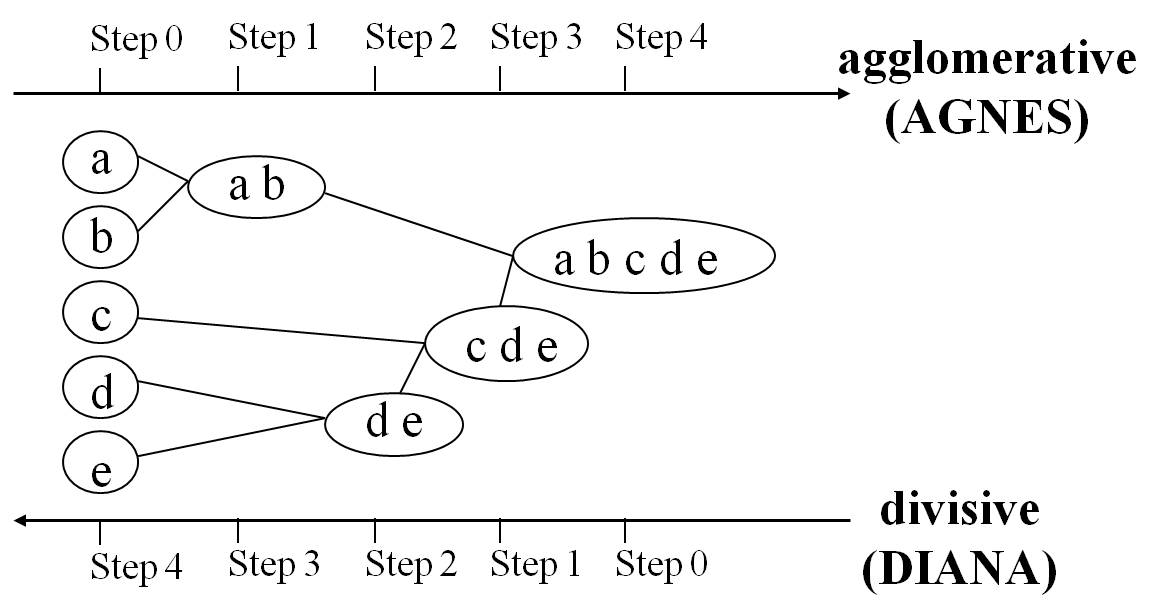
\includegraphics{figures/hierarchical.jpg}
\end{frame}



\begin{frame}[fragile, plain]{Hierarchical clustering}
\textbf{Distance}
\begin{itemize}
 \item Continuous variables: euclidean, manhattan, canberra, ...
 \item Categorical variables: binary
 \item Mixed variables: Gower   
\end{itemize}
\end{frame}


%%%%%%%%%%%%%%%%%%%%%%%%%%%%%%%%%%%
\subsection{Partitioning methods}
%%%%%%%%%%%%%%%%%%%%%%%%%%%%%%%%%%%

\begin{frame}[fragile, plain]{Partitioning methods}
Construct a partition of a database into a set of k clusters

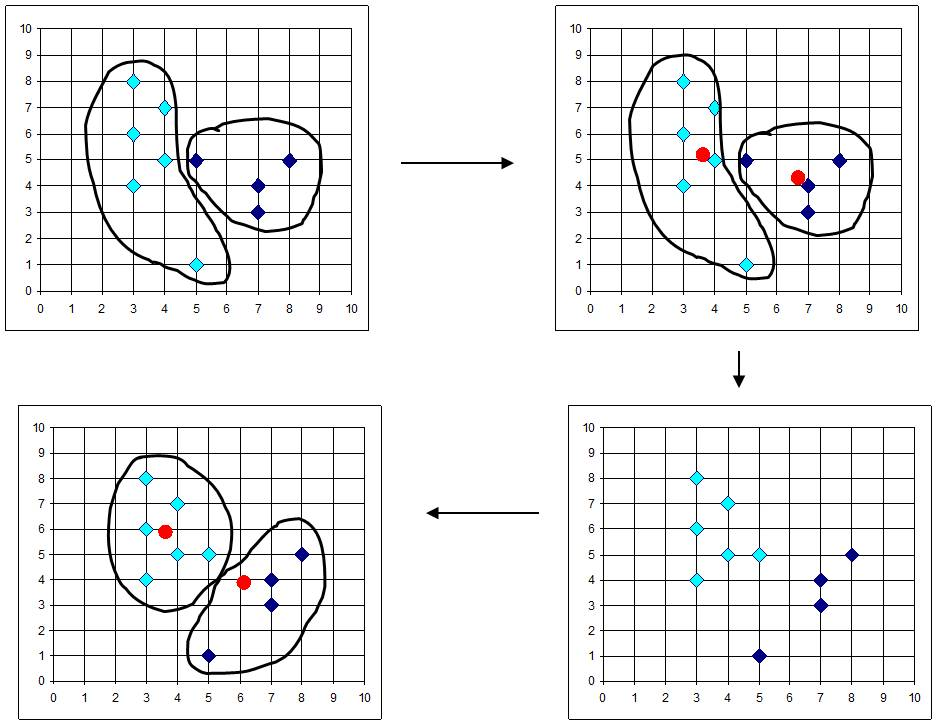
\includegraphics{figures/kmeans.jpg}
\end{frame}


\begin{frame}[fragile, plain]{Partitioning methods}
\begin{itemize}
\item Strengths
  \begin{itemize}
   \item Relatively efficient O(nk) 
   \item Often ends at a local optimum
  \end{itemize}
\item Weeknesses
 \begin{itemize}
   \item Applicable only when mean is define - what about categorical data?
   \item Need to specify $k$, the number of clusters, in advance
   \item Unable to handle noisy data and outliers
   \item Non suitable to discover clusters with non-convex shapes
  \end{itemize}

\end{itemize}


\end{frame}



\begin{frame}[fragile, plain]{Partitioning methods: k-medoids}
\begin{itemize}
\item Find representative (i.e., the most centrally located) objects, called medoids, in clusters
\item PAM (Partitioning Around Medoids)
  \begin{itemize}
    \item starts from a initial set of medoids and iteratively replaces one of the medoids by one of the non-medoids when 
        total distance is improved in the resulting clustering
    \item works fine for small data sets
    \item more robust than k-means
    \item more complex: $O(k(n-k)^2)$
 \end{itemize}
\item CLARA: Uses multiple samples
\item CLARANS: Randomized sampling
 \end{itemize}


\end{frame}


%%%%%%%%%%%%%%%%%%%%%%%%%%%%%%%%%%%
\subsection{Model-based methods}
%%%%%%%%%%%%%%%%%%%%%%%%%%%%%%%%%%%

\begin{frame}[fragile, plain]{Model-based methods}
$$ f(x) = \sum_{g=1}^G \pi_G \phi(x | \mu_g, \Sigma_g) $$

where $\pi_g$ is the probability that an observation belongs to group $g$ and
$\phi(x | \mu_g, \Sigma_g)$ is the density of a multivariate Gaussian.
\begin{itemize}
 \item MCLUST
 \item Latent class approach
\end{itemize}
\end{frame}


%%%%%%%%%%%%%%%%%%%%%%%%%%%%%%%%%%%
\subsection{Clusteing methods with R}
%%%%%%%%%%%%%%%%%%%%%%%%%%%%%%%%%%%


\begin{frame}[fragile, plain]{Clustering methods with R}
\textbf{Example}: To illustrate interpretation of different Clustering methods, we'll look at 
a cluster analysis performed on a set of cars from 1978-1979; the data can be found at 
http://www.stat.berkeley.edu/classes/s133/data/cars.tab. Since the data is a tab-delimited file, we use read.delim:

\begin{knitrout}\footnotesize
\definecolor{shadecolor}{rgb}{0.969, 0.969, 0.969}\color{fgcolor}\begin{kframe}
\begin{alltt}
\hlstd{dd} \hlkwb{<-} \hlkwd{read.delim}\hlstd{(}\hlstr{"data/cars.tab"}\hlstd{)}
\hlkwd{head}\hlstd{(dd)}
\end{alltt}
\begin{verbatim}
##   Country                       Car  MPG Weight Drive_Ratio Horsepower
## 1    U.S.        Buick Estate Wagon 16.9  4.360        2.73        155
## 2    U.S. Ford Country Squire Wagon 15.5  4.054        2.26        142
## 3    U.S.        Chevy Malibu Wagon 19.2  3.605        2.56        125
## 4    U.S.    Chrysler LeBaron Wagon 18.5  3.940        2.45        150
## 5    U.S.                  Chevette 30.0  2.155        3.70         68
## 6   Japan             Toyota Corona 27.5  2.560        3.05         95
##   Displacement Cylinders
## 1          350         8
## 2          351         8
## 3          267         8
## 4          360         8
## 5           98         4
## 6          134         4
\end{verbatim}
\end{kframe}
\end{knitrout}

\end{frame}

\begin{frame}[fragile, plain]{Data scalling}
It looks like the variable are measured on different scales. This requires data standardization.We will apply 'robust' normalization (scale can also be used). There are functions like
{\tt daisy} from {\tt cluster} package that will automatically perform standardization, but it doesn't give you complete control.

\begin{knitrout}\footnotesize
\definecolor{shadecolor}{rgb}{0.969, 0.969, 0.969}\color{fgcolor}\begin{kframe}
\begin{alltt}
\hlstd{dd.ok} \hlkwb{<-} \hlstd{dd[ ,} \hlopt{-}\hlkwd{c}\hlstd{(}\hlnum{1}\hlstd{,}\hlnum{2}\hlstd{)]}
\hlstd{medians} \hlkwb{<-} \hlkwd{apply}\hlstd{(dd.ok,} \hlnum{2}\hlstd{, median)}
\hlstd{mads} \hlkwb{<-} \hlkwd{apply}\hlstd{(dd.ok,} \hlnum{2}\hlstd{, mad)} \hlcom{# median absolute deviation}
\hlstd{dd.ok} \hlkwb{<-} \hlkwd{scale}\hlstd{(dd.ok,} \hlkwc{center}\hlstd{=medians,} \hlkwc{scale}\hlstd{=mads)}
\end{alltt}
\end{kframe}
\end{knitrout}
\end{frame}


\begin{frame}[fragile, plain]{Hiherarchical methods}

\begin{knitrout}\footnotesize
\definecolor{shadecolor}{rgb}{0.969, 0.969, 0.969}\color{fgcolor}\begin{kframe}
\begin{alltt}
\hlstd{dd.dist} \hlkwb{<-} \hlkwd{dist}\hlstd{(dd.ok)}
\hlstd{dd.dist.camb} \hlkwb{<-} \hlkwd{dist}\hlstd{(dd.ok,} \hlkwc{method}\hlstd{=}\hlstr{"canberra"}\hlstd{)}
\end{alltt}
\end{kframe}
\end{knitrout}

\begin{knitrout}\footnotesize
\definecolor{shadecolor}{rgb}{0.969, 0.969, 0.969}\color{fgcolor}\begin{kframe}
\begin{alltt}
\hlkwd{library}\hlstd{(cluster)}
\hlstd{dd.dist.gower} \hlkwb{<-} \hlkwd{daisy}\hlstd{(dd.ok,} \hlkwc{metric}\hlstd{=}\hlstr{"gower"}\hlstd{)}
\end{alltt}
\end{kframe}
\end{knitrout}

\end{frame}


\begin{frame}[fragile, plain]{Hiherarchical methods}
Dendogram is the main graphical tool for getting insight into a cluster solution

\begin{knitrout}\footnotesize
\definecolor{shadecolor}{rgb}{0.969, 0.969, 0.969}\color{fgcolor}\begin{kframe}
\begin{alltt}
\hlstd{dd.hclust} \hlkwb{<-} \hlkwd{hclust}\hlstd{(dd.dist)}
\hlkwd{plot}\hlstd{(dd.hclust,} \hlkwc{labels}\hlstd{=dd}\hlopt{$}\hlstd{Car,} \hlkwc{main}\hlstd{=}\hlstr{""}\hlstd{)}
\end{alltt}
\end{kframe}

{\centering 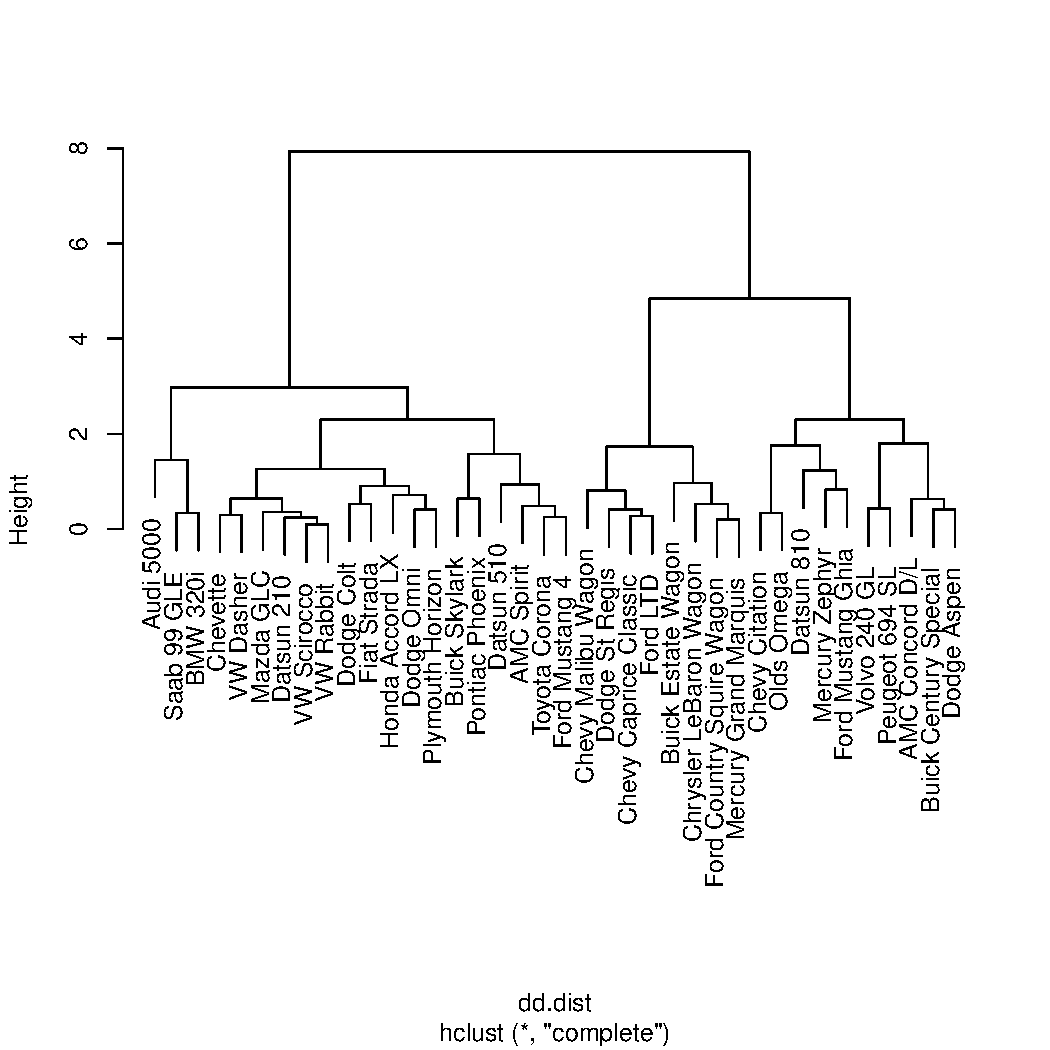
\includegraphics[width=2in]{figure/hclust-1} 

}



\end{knitrout}
\end{frame}

\begin{frame}[fragile, plain]{Hiherarchical methods}
One may be interested in knowing how many samples/features are in each group that is defined by 
a given height along the y-axis.  

\begin{knitrout}\footnotesize
\definecolor{shadecolor}{rgb}{0.969, 0.969, 0.969}\color{fgcolor}\begin{kframe}
\begin{alltt}
\hlstd{groups3.hclust} \hlkwb{<-} \hlkwd{as.factor}\hlstd{(}\hlkwd{cutree}\hlstd{(dd.hclust,} \hlnum{3}\hlstd{))}
\hlkwd{table}\hlstd{(groups3.hclust)}
\end{alltt}
\begin{verbatim}
## groups3.hclust
##  1  2  3 
##  8 20 10
\end{verbatim}
\end{kframe}
\end{knitrout}
\end{frame}

\begin{frame}[fragile, plain]{Hiherarchical methods}
To see which individuals/features are in each group ...

\begin{knitrout}\footnotesize
\definecolor{shadecolor}{rgb}{0.969, 0.969, 0.969}\color{fgcolor}\begin{kframe}
\begin{alltt}
\hlstd{dd}\hlopt{$}\hlstd{Car[groups3.hclust}\hlopt{==}\hlnum{1}\hlstd{]}
\end{alltt}
\begin{verbatim}
## [1] Buick Estate Wagon        Ford Country Squire Wagon
## [3] Chevy Malibu Wagon        Chrysler LeBaron Wagon   
## [5] Chevy Caprice Classic     Ford LTD                 
## [7] Mercury Grand Marquis     Dodge St Regis           
## 38 Levels: AMC Concord D/L AMC Spirit Audi 5000 ... VW Scirocco
\end{verbatim}
\end{kframe}
\end{knitrout}


To see which individuals/features are in each group ...

\begin{knitrout}\footnotesize
\definecolor{shadecolor}{rgb}{0.969, 0.969, 0.969}\color{fgcolor}\begin{kframe}
\begin{alltt}
\hlkwd{sapply}\hlstd{(}\hlkwd{unique}\hlstd{(groups3.hclust),} \hlkwa{function} \hlstd{(}\hlkwc{x}\hlstd{) dd}\hlopt{$}\hlstd{Car[groups3.hclust}\hlopt{==}\hlstd{x])}
\end{alltt}
\begin{verbatim}
## [[1]]
## [1] Buick Estate Wagon        Ford Country Squire Wagon
## [3] Chevy Malibu Wagon        Chrysler LeBaron Wagon   
## [5] Chevy Caprice Classic     Ford LTD                 
## [7] Mercury Grand Marquis     Dodge St Regis           
## 38 Levels: AMC Concord D/L AMC Spirit Audi 5000 ... VW Scirocco
## 
## [[2]]
##  [1] Chevette         Toyota Corona    Datsun 510       Dodge Omni      
##  [5] Audi 5000        Saab 99 GLE      Ford Mustang 4   Mazda GLC       
##  [9] Dodge Colt       AMC Spirit       VW Scirocco      Honda Accord LX 
## [13] Buick Skylark    Pontiac Phoenix  Plymouth Horizon Datsun 210      
## [17] Fiat Strada      VW Dasher        BMW 320i         VW Rabbit       
## 38 Levels: AMC Concord D/L AMC Spirit Audi 5000 ... VW Scirocco
## 
## [[3]]
##  [1] Volvo 240 GL          Peugeot 694 SL        Buick Century Special
##  [4] Mercury Zephyr        Dodge Aspen           AMC Concord D/L      
##  [7] Ford Mustang Ghia     Chevy Citation        Olds Omega           
## [10] Datsun 810           
## 38 Levels: AMC Concord D/L AMC Spirit Audi 5000 ... VW Scirocco
\end{verbatim}
\end{kframe}
\end{knitrout}
\end{frame}


\begin{frame}[fragile, plain]{Hiherarchical methods}
Dendrogram can be colour
\begin{knitrout}\footnotesize
\definecolor{shadecolor}{rgb}{0.969, 0.969, 0.969}\color{fgcolor}\begin{kframe}
\begin{alltt}
\hlstd{dend} \hlkwb{<-} \hlkwd{as.dendrogram}\hlstd{(dd.hclust)}
\hlstd{dend2} \hlkwb{<-} \hlstd{dendextend}\hlopt{::}\hlkwd{color_labels}\hlstd{(dend,} \hlkwc{k}\hlstd{=}\hlnum{3}\hlstd{)}
\hlstd{dendextend}\hlopt{::}\hlkwd{labels}\hlstd{(dend2)} \hlkwb{<-} \hlstd{dd}\hlopt{$}\hlstd{Car}
\hlkwd{plot}\hlstd{(dend2)}
\end{alltt}
\end{kframe}

{\centering 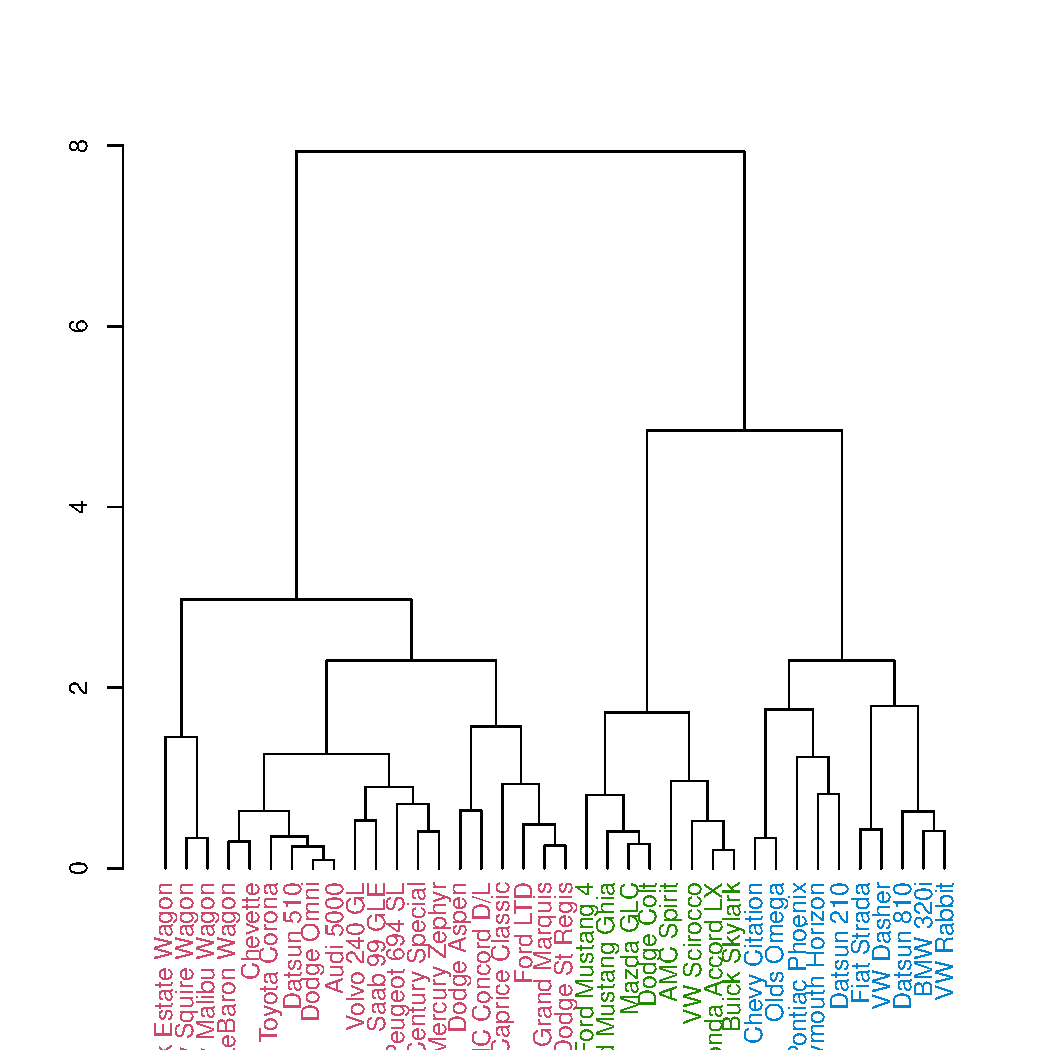
\includegraphics[width=2in]{figure/hclustCol-1} 

}



\end{knitrout}
\end{frame}


\begin{frame}[fragile, plain]{Partitioning methods}
\begin{knitrout}\footnotesize
\definecolor{shadecolor}{rgb}{0.969, 0.969, 0.969}\color{fgcolor}\begin{kframe}
\begin{alltt}
\hlkwd{require}\hlstd{(cluster)}
\hlstd{dd.pam} \hlkwb{<-} \hlkwd{pam}\hlstd{(dd.dist,} \hlnum{3}\hlstd{)}
\hlstd{dd.kmeans} \hlkwb{<-} \hlkwd{kmeans}\hlstd{(dd.dist,} \hlnum{3}\hlstd{)}
\hlstd{groups3.pam} \hlkwb{<-} \hlkwd{as.factor}\hlstd{(dd.pam}\hlopt{$}\hlstd{clustering)}
\hlstd{groups3.kmeans} \hlkwb{<-}  \hlkwd{as.factor}\hlstd{(dd.kmeans}\hlopt{$}\hlstd{cluster)}
\end{alltt}
\end{kframe}
\end{knitrout}

\end{frame}



\begin{frame}[fragile, plain]{Partitioning methods}
\begin{knitrout}\footnotesize
\definecolor{shadecolor}{rgb}{0.969, 0.969, 0.969}\color{fgcolor}\begin{kframe}
\begin{alltt}
\hlkwd{table}\hlstd{(groups3.pam, groups3.hclust)}
\end{alltt}
\begin{verbatim}
##            groups3.hclust
## groups3.pam  1  2  3
##           1  8  0  0
##           2  0 19  0
##           3  0  1 10
\end{verbatim}
\begin{alltt}
\hlkwd{table}\hlstd{(groups3.pam, groups3.kmeans)}
\end{alltt}
\begin{verbatim}
##            groups3.kmeans
## groups3.pam  1  2  3
##           1  0  8  0
##           2 19  0  0
##           3  0  0 11
\end{verbatim}
\end{kframe}
\end{knitrout}

\end{frame}


\begin{frame}[fragile, plain]{Partitioning methods}
Silhouette plot describe how good the structure of the clusters is.
\begin{knitrout}\footnotesize
\definecolor{shadecolor}{rgb}{0.969, 0.969, 0.969}\color{fgcolor}\begin{kframe}
\begin{alltt}
\hlkwd{plot}\hlstd{(dd.pam)}
\end{alltt}
\end{kframe}

{\centering 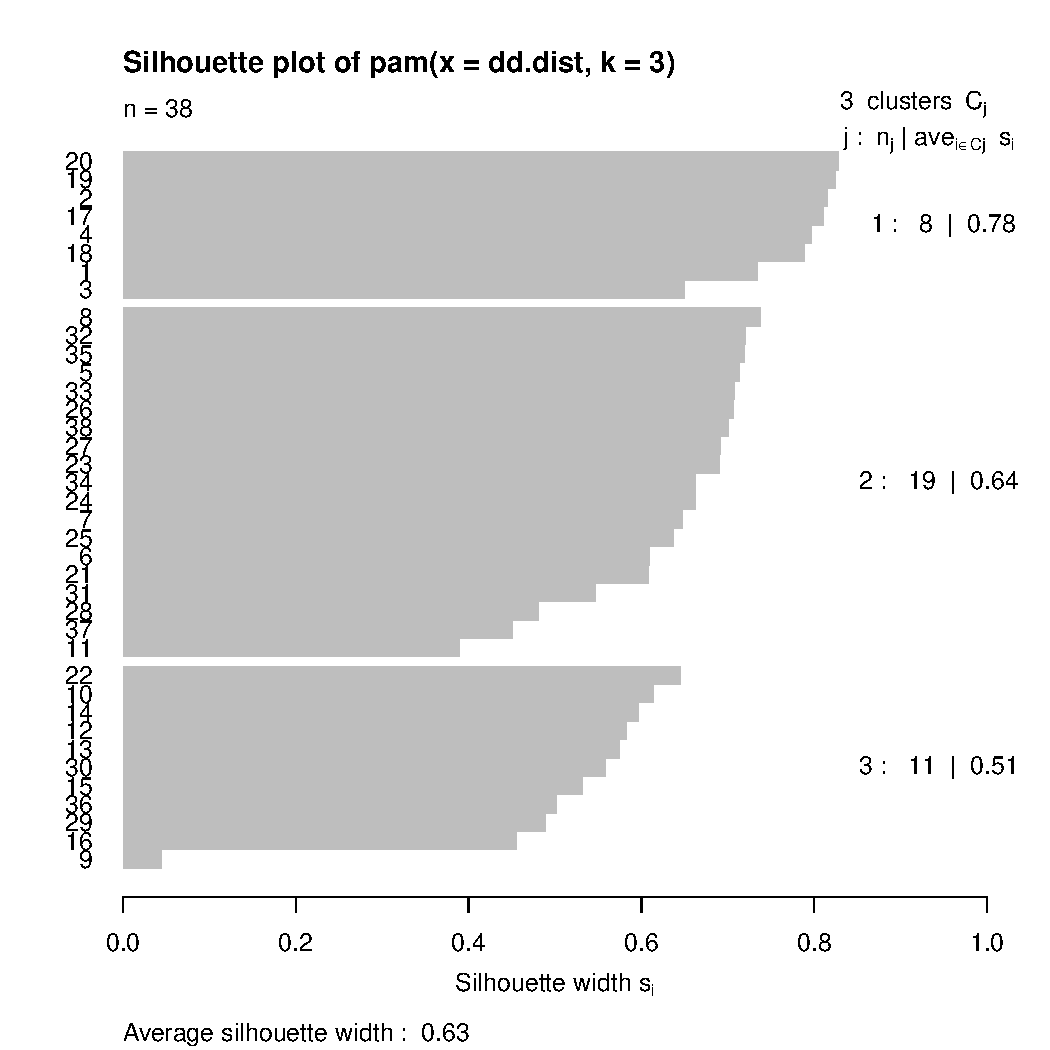
\includegraphics[width=2in]{figure/pamPlot-1} 

}



\end{knitrout}

\end{frame}

\begin{frame}[fragile, plain]{Partitioning methods}
There is a criteria to interpret these values

\begin{table}[h]
\begin{tabular}{ll}
\hline \hline
Range of SC & Interpretation                                \\
\hline
0.71-1.00   & A strong structure has been found             \\
0.51-0.70   & A reasonable structure has been found         \\
0.26-0.50   & The structure is weak and could be artificial \\
0-0.25      & No substantial structure has been found      \\
\hline \hline
\end{tabular}
\end{table}

\end{frame}

\begin{frame}[fragile, plain]{Partitioning methods}
Silhouette plot can be created for any method
\begin{knitrout}\footnotesize
\definecolor{shadecolor}{rgb}{0.969, 0.969, 0.969}\color{fgcolor}\begin{kframe}
\begin{alltt}
\hlkwd{plot}\hlstd{(}\hlkwd{silhouette}\hlstd{(}\hlkwd{cutree}\hlstd{(dd.hclust,}\hlnum{4}\hlstd{), dd.dist))}
\end{alltt}
\end{kframe}

{\centering 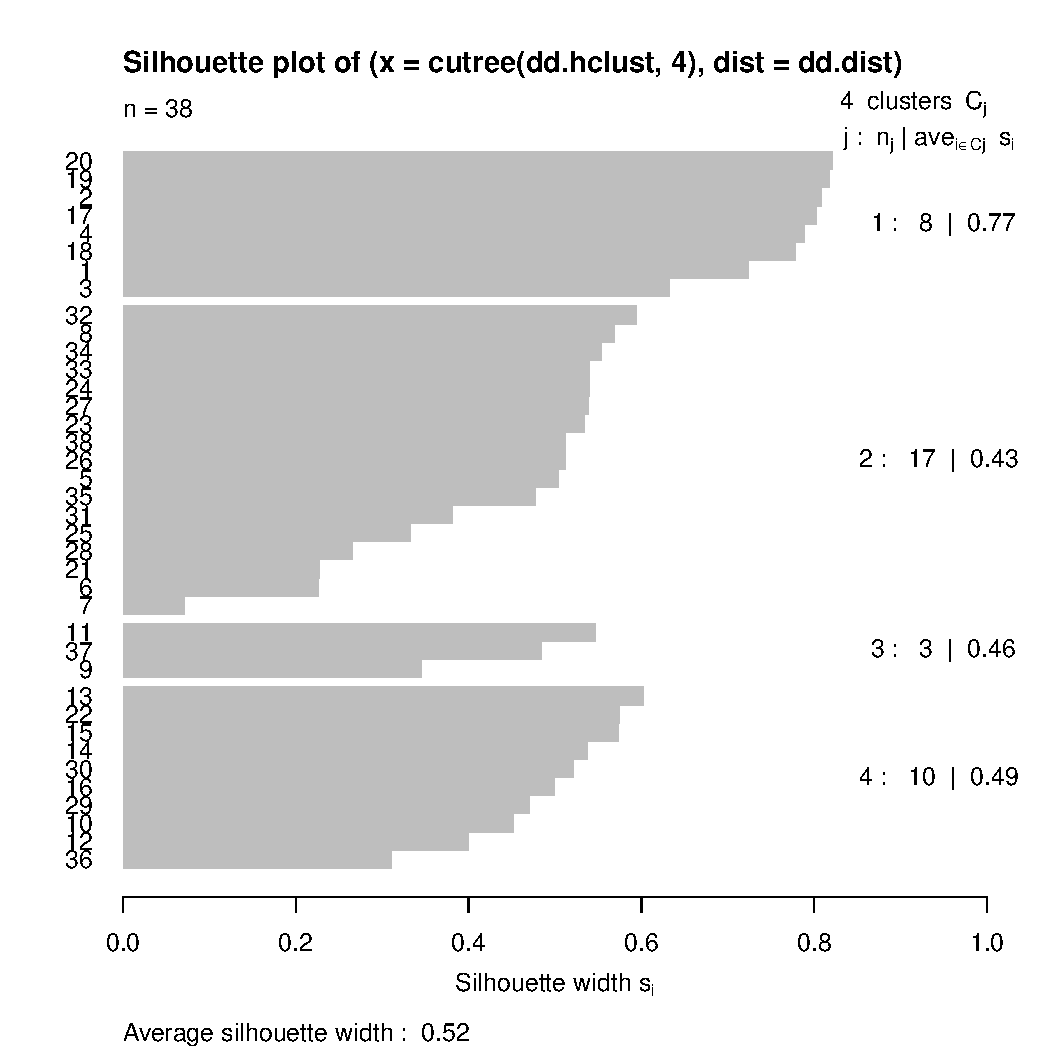
\includegraphics[width=2in]{figure/pamPlotAny-1} 

}



\end{knitrout}

\end{frame}


\begin{frame}[fragile, plain]{Model-based}
Mclust assumes Multivariate Gaussian distribution
\begin{knitrout}\footnotesize
\definecolor{shadecolor}{rgb}{0.969, 0.969, 0.969}\color{fgcolor}\begin{kframe}
\begin{alltt}
\hlkwd{require}\hlstd{(mclust)}
\hlstd{dd.mclust} \hlkwb{<-} \hlkwd{Mclust}\hlstd{(dd.ok)}
\hlkwd{summary}\hlstd{(dd.mclust)}
\end{alltt}
\begin{verbatim}
## ----------------------------------------------------
## Gaussian finite mixture model fitted by EM algorithm 
## ----------------------------------------------------
## 
## Mclust VEV (ellipsoidal, equal shape) model with 6 components:
## 
##  log.likelihood  n  df      BIC      ICL
##        293.5089 38 142 70.48055 70.47931
## 
## Clustering table:
##  1  2  3  4  5  6 
##  8  6 10  7  5  2
\end{verbatim}
\end{kframe}
\end{knitrout}
\end{frame}




\begin{frame}[fragile, plain]{Model-based}
Mclust assumes Multivariate Gaussian distribution
\begin{knitrout}\footnotesize
\definecolor{shadecolor}{rgb}{0.969, 0.969, 0.969}\color{fgcolor}\begin{kframe}
\begin{alltt}
\hlstd{groups3.mclust} \hlkwb{<-} \hlkwd{Mclust}\hlstd{(dd.ok,} \hlkwc{G}\hlstd{=}\hlnum{3}\hlstd{)}\hlopt{$}\hlstd{class}
\hlkwd{table}\hlstd{(groups3.mclust, groups3.pam)}
\end{alltt}
\begin{verbatim}
##               groups3.pam
## groups3.mclust  1  2  3
##              1  8  0  0
##              2  0 19  0
##              3  0  0 11
\end{verbatim}
\end{kframe}
\end{knitrout}
\end{frame}



\begin{frame}[fragile, plain]{Model-based}

\begin{knitrout}\footnotesize
\definecolor{shadecolor}{rgb}{0.969, 0.969, 0.969}\color{fgcolor}\begin{kframe}
\begin{alltt}
\hlkwd{mclust2Dplot}\hlstd{(dd.ok[,}\hlnum{1}\hlopt{:}\hlnum{2}\hlstd{],} \hlkwc{parameters}\hlstd{=dd.mclust}\hlopt{$}\hlstd{parameters,}
             \hlkwc{z}\hlstd{=dd.mclust}\hlopt{$}\hlstd{z,} \hlkwc{what} \hlstd{=} \hlstr{"classification"}\hlstd{)}
\end{alltt}
\end{kframe}

{\centering 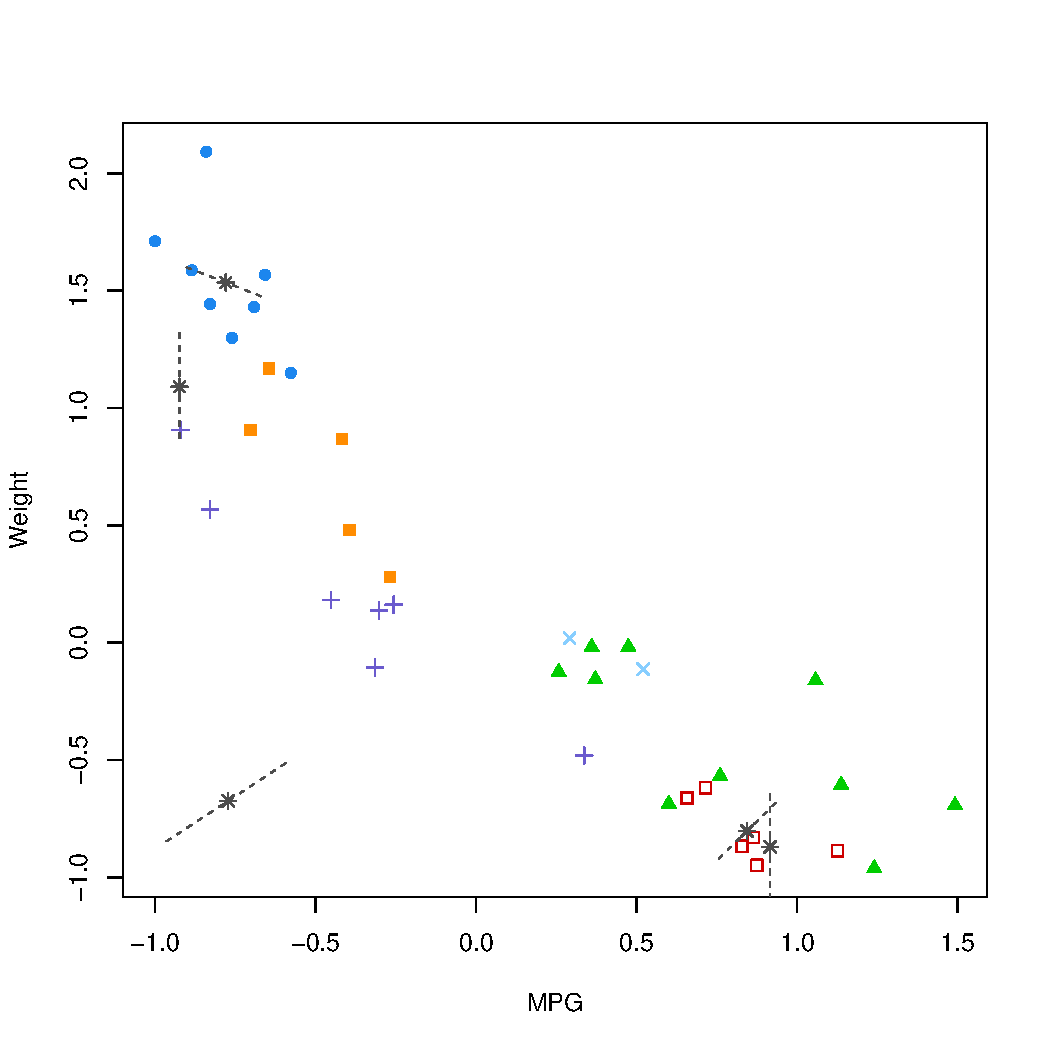
\includegraphics[width=2in]{figure/mclustFig2D-1} 

}



\end{knitrout}

\end{frame}


%%%%%%%%%%%%%%%%%%%%%%%%%%%%%%%%%%%
\section{Clustering related issues}
%%%%%%%%%%%%%%%%%%%%%%%%%%%%%%%%%%%

\begin{frame}[fragile, plain]{Clustering related issues}
Key issues
\begin{itemize}
 \item Number of clusters?
 \item Are clusters statistically significant?
 \item Are clusters reproducible? 
 \item Big datasets?
 \item Sparse data in genomics? 
\end{itemize}

\end{frame}

\begin{frame}[fragile, plain]{Number of clusters}

\begin{itemize}
 \item Model-based: AIC
 \item Clustering methods: 
 \begin{itemize}
  \item \textbf{calinski}: (SSB/(K-1))/(SSW/(n-K)), where n is the number of data points and K is the number of clusters. 
               SSW is the sum of squares within the clusters while SSB is the sum of squares among the clusters. 
               This index is simply an F (ANOVA) statistic.
  \item \textbf{ssi}: the \emph{Simple Structure Index} multiplicatively combines several elements which influence the 
                      interpretability of a partitioning solution. The best partition is indicated by the highest 
                      SSI value.
 \end{itemize} 
\end{itemize}

\end{frame}

\begin{frame}[fragile, plain]{Number of clusters}

\begin{knitrout}\footnotesize
\definecolor{shadecolor}{rgb}{0.969, 0.969, 0.969}\color{fgcolor}\begin{kframe}
\begin{alltt}
\hlkwd{require}\hlstd{(vegan)}
\hlstd{k.cal} \hlkwb{<-} \hlkwd{cascadeKM}\hlstd{(dd.ok,} \hlkwc{inf.gr}\hlstd{=}\hlnum{2}\hlstd{,} \hlkwc{sup.gr}\hlstd{=}\hlnum{6}\hlstd{,} \hlkwc{criterion}\hlstd{=}\hlstr{"calinski"}\hlstd{)}
\hlstd{k.ssi} \hlkwb{<-} \hlkwd{cascadeKM}\hlstd{(dd.ok,} \hlkwc{inf.gr}\hlstd{=}\hlnum{2}\hlstd{,} \hlkwc{sup.gr}\hlstd{=}\hlnum{6}\hlstd{,} \hlkwc{criterion}\hlstd{=}\hlstr{"ssi"}\hlstd{)}
\end{alltt}
\end{kframe}
\end{knitrout}

\end{frame}


\begin{frame}[fragile, plain]{Number of clusters}

\begin{knitrout}\footnotesize
\definecolor{shadecolor}{rgb}{0.969, 0.969, 0.969}\color{fgcolor}\begin{kframe}
\begin{alltt}
\hlkwd{plot}\hlstd{(k.cal)}
\end{alltt}
\end{kframe}

{\centering 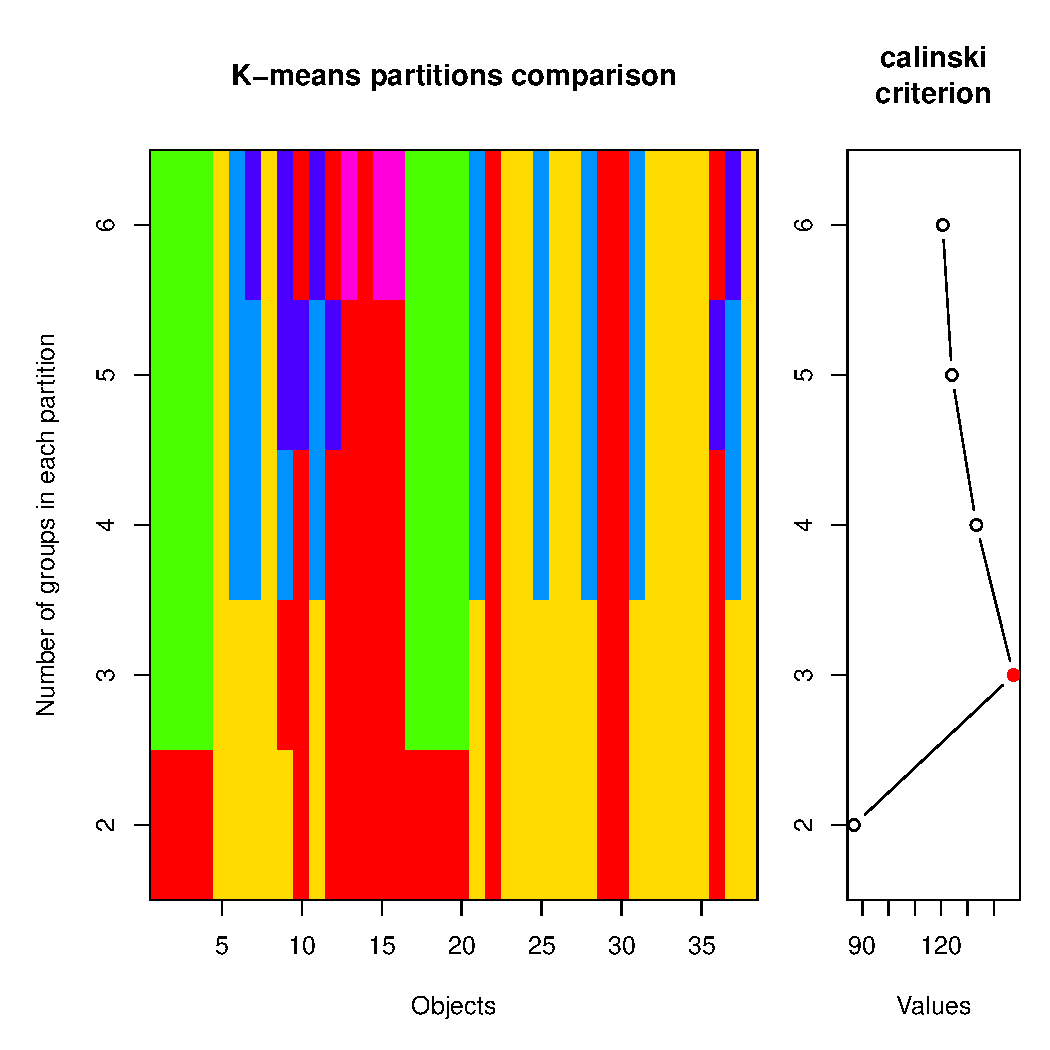
\includegraphics[width=2in]{figure/plotCal-1} 

}



\end{knitrout}

\end{frame}


\begin{frame}[fragile, plain]{Number of clusters}

\begin{knitrout}\footnotesize
\definecolor{shadecolor}{rgb}{0.969, 0.969, 0.969}\color{fgcolor}\begin{kframe}
\begin{alltt}
\hlkwd{plot}\hlstd{(k.ssi)}
\end{alltt}
\end{kframe}

{\centering 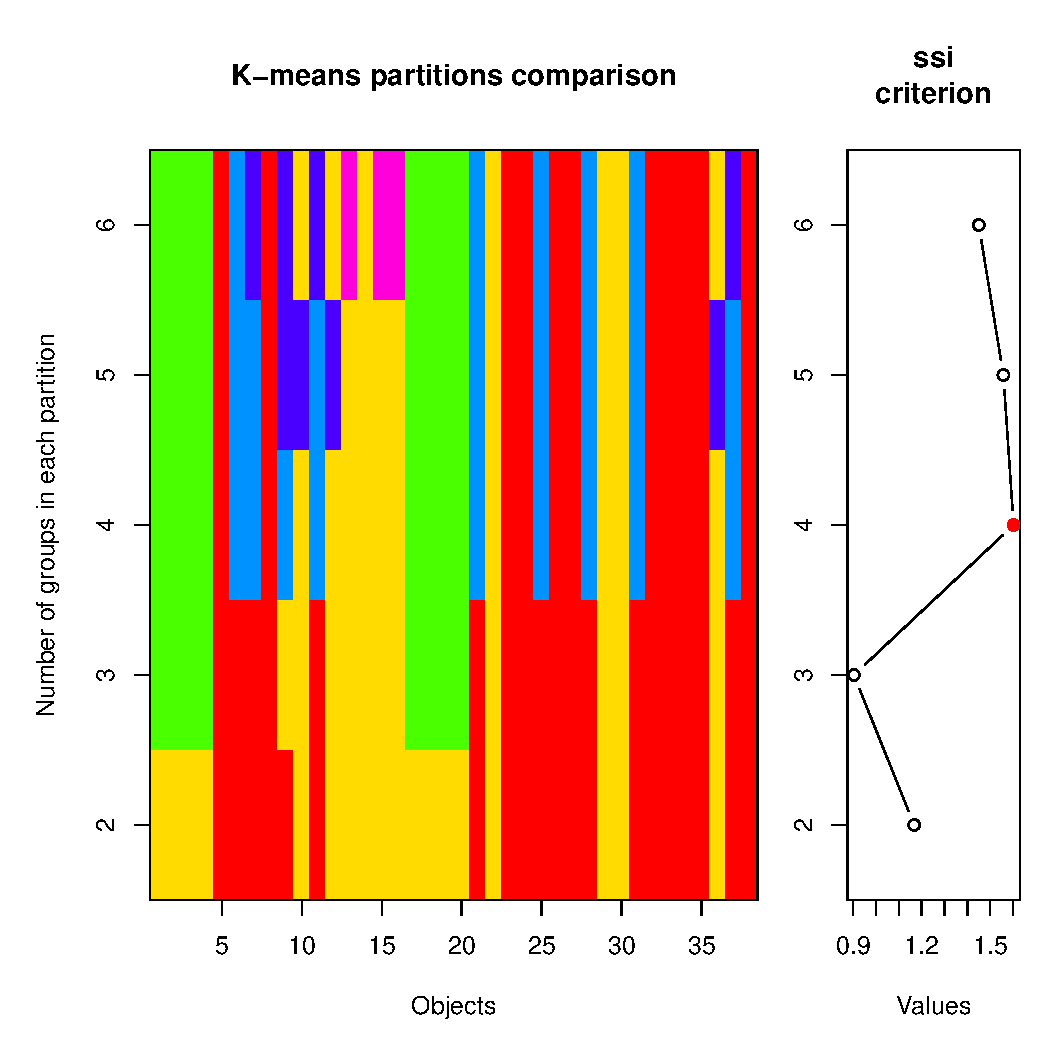
\includegraphics[width=2in]{figure/plotSsi-1} 

}



\end{knitrout}

\end{frame}


\begin{frame}[fragile, plain]{Testing clustering results}

Test for 2 clusters vs 1 

\begin{knitrout}\footnotesize
\definecolor{shadecolor}{rgb}{0.969, 0.969, 0.969}\color{fgcolor}\begin{kframe}
\begin{alltt}
\hlkwd{require}\hlstd{(sigclust)}
\hlstd{mod.sig} \hlkwb{<-}\hlkwd{sigclust}\hlstd{(dd.ok,} \hlkwc{nsim}\hlstd{=}\hlnum{1000}\hlstd{)}
\hlkwd{plot}\hlstd{(mod.sig,} \hlkwc{arg}\hlstd{=}\hlstr{"pvalue"}\hlstd{)}
\end{alltt}
\end{kframe}

{\centering 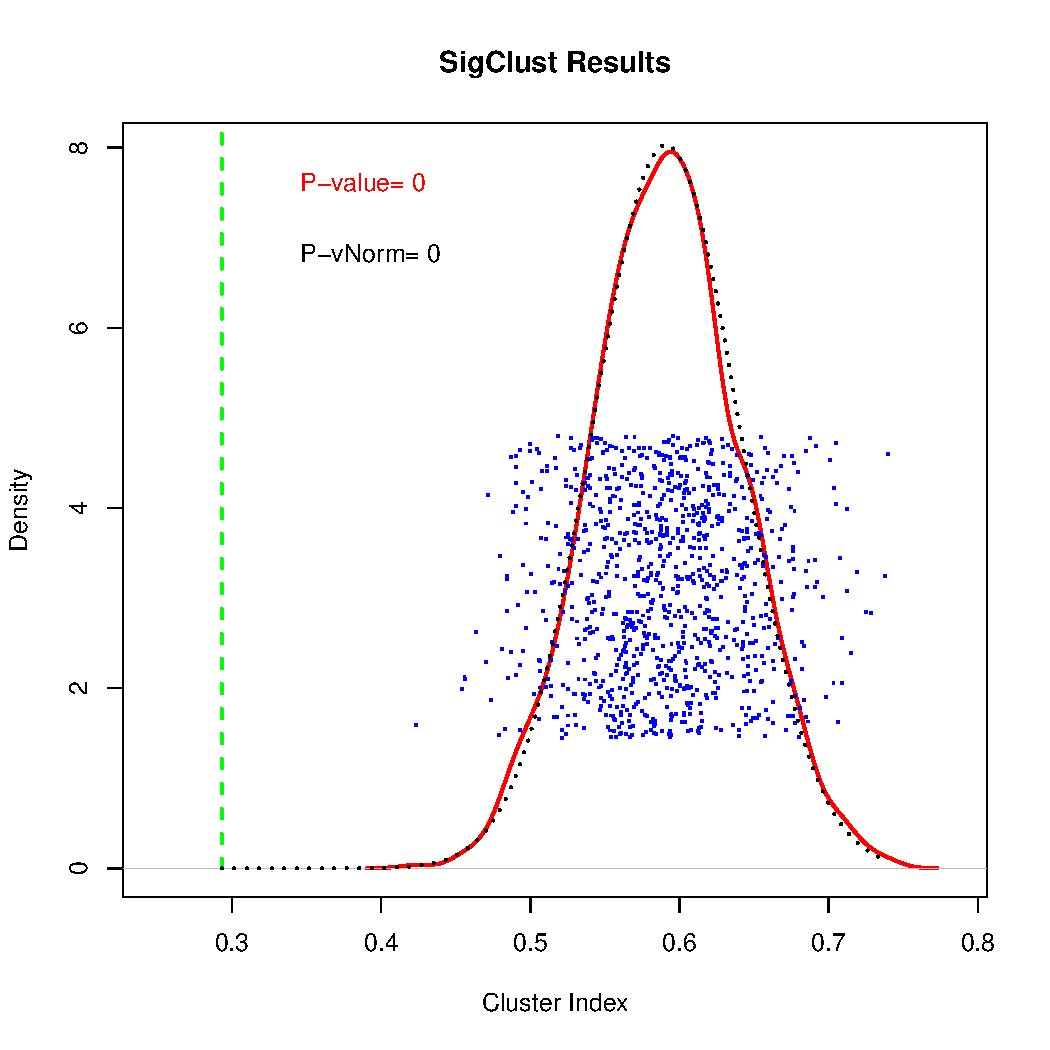
\includegraphics[width=2in]{figure/plotTest-1} 

}



\end{knitrout}

\end{frame}


\begin{frame}[fragile, plain]{Cluster validation}
\begin{knitrout}\footnotesize
\definecolor{shadecolor}{rgb}{0.969, 0.969, 0.969}\color{fgcolor}\begin{kframe}
\begin{alltt}
\hlkwd{require}\hlstd{(clValid)}
\hlstd{val.intern} \hlkwb{<-} \hlkwd{clValid}\hlstd{(dd.ok,} \hlnum{2}\hlopt{:}\hlnum{6}\hlstd{,} \hlkwc{clMethods} \hlstd{=} \hlkwd{c}\hlstd{(}\hlstr{"hierarchical"}\hlstd{,}
 \hlstr{"kmeans"}\hlstd{,} \hlstr{"diana"}\hlstd{,} \hlstr{"pam"}\hlstd{,}  \hlstr{"model"}\hlstd{),} \hlkwc{validation} \hlstd{=} \hlstr{"internal"}\hlstd{)}
\hlkwd{optimalScores}\hlstd{(val.intern)}
\end{alltt}
\begin{verbatim}
##                  Score       Method Clusters
## Connectivity 2.6317460       kmeans        2
## Dunn         0.5619325 hierarchical        2
## Silhouette   0.6297805       kmeans        3
\end{verbatim}
\end{kframe}
\end{knitrout}
\end{frame}

\begin{frame}[fragile, plain]{Big datasets}
\begin{knitrout}\footnotesize
\definecolor{shadecolor}{rgb}{0.969, 0.969, 0.969}\color{fgcolor}\begin{kframe}
\begin{alltt}
\hlkwd{require}\hlstd{(fastcluster)}
\hlstd{hclust.fast} \hlkwb{<-} \hlkwd{hclust}\hlstd{(dd.dist)}
\end{alltt}
\end{kframe}
\end{knitrout}
\end{frame}

\end{document}





